\documentclass[twoside,bibtotoc]{report}

% ------
% Umlaute
\usepackage{ifluatex,ifxetex}
\ifluatex
  \usepackage{fontspec}
\else
  \ifxetex
    \usepackage{fontspec}
  \else
    \usepackage{selinput}
    \SelectInputMappings{
      adieresis={ä},
      germandbls={ß},
    }
    \usepackage[T1]{fontenc}
    %\usepackage{textcomp}% optional
    %\usepackage{lmodern}
  \fi
\fi

% ------
% Paper auf Deutsch
\usepackage[ngerman]{babel}
%\usepackage[english]{babel}

% ------
% Page layout
\usepackage[hmarginratio=1:1,top=32mm,columnsep=20pt]{geometry}
\usepackage[font=it]{caption}
\usepackage{paralist}
%\usepackage{multicol}

% ------
% Titling (section/subsection)
\usepackage{titlesec}
\renewcommand\thesection{\arabic{section}}
\titleformat{\section}[block]{\Large\scshape\bfseries}{\thesection.}{1em}{}
\setcounter{secnumdepth}{3}

% ------
% Zeichenfunktionen
\usepackage{pgfplots}
\pgfplotsset{compat=1.8}
\usepgfplotslibrary{statistics}
\usetikzlibrary{patterns}

\usepackage{float}


%%%%%%%%%%%%%%%%%%%%%%%%%%%%%%%%%%%%%%%%%%%%%%%%%%%%%%%%%%%%%%%%%%%%%%%%%%%%%%
%Titelseite
\title{\textbf{Evolutionäre Algorithmen Projekt - ''Circle Packing''}}
%\footnotesize{Lizenz: CC BY-NC}}

\author{
Valentin Felder - valentin.felder@stud.htwk-leipzig.de
}
\date{\today}


%%%%%%%%%%%%%%%%%%%%%%%%%%%%%%%%%%%%%%%%%%%%%%%%%%%%%%%%%%%%%%%%%%%%%%%%%%%%%%
% ------
% Clickable URLs (optional)
%\usepackage{hyperref}
\usepackage[colorlinks=true,linkcolor=black]{hyperref} %Verlinkung des Inhaltsverzeichnisses ohne roten Rahmen um den Text
\hypersetup{colorlinks=blue, citecolor=blue,filecolor=blue,linkcolor=blue,urlcolor=red} %Einfärbung
%\hypersetup{colorlinks=black, citecolor=black,filecolor=black,linkcolor=black,urlcolor=black} %Einfärbung sonstiger links


%Grafik-Elemente
\usepackage{graphicx}
\usepackage{amsmath}
\usepackage{amssymb}
\usepackage{textcomp}
\usepackage{gensymb}
%\usepackage[latin1]{inputenc}
%\usepackage[T1]{fontenc}


\usepackage[backend=bibtex]{biblatex} %Zitate verwenden
\bibliography{lit.bib} %Pfad zu den Quellen


\usepackage{caption}
\usepackage{tikz}


% Erweiterte Tabellen
\usepackage{tabularx}
\usepackage{multirow}
\usepackage{float}
\restylefloat{table}

%Tabellen mit Items
\usepackage{booktabs}% http://ctan.org/pkg/booktabs
\newcommand{\tabitem}{~~\llap{\textbullet}~~}


% Code Beispiel C++
\usepackage{listings}
\lstset{
	language=C++,
	aboveskip=2mm,
	belowskip=2mm,
	showstringspaces=false,
	columns=flexible,
	basicstyle={\small\ttfamily},
	numbers=none,
	breaklines=true,
	breakatwhitespace=true,
	tabsize=3
}


%\usepackage{listings}
\usepackage{color}
\definecolor{cGray}{rgb}{0.5,0.5,0.5}
\definecolor{cGreen}{RGB}{0, 132, 8}
\definecolor{cBlue}{RGB}{31, 93, 193}
\definecolor{cPink}{RGB}{204, 0, 219}
\definecolor{cOrange}{RGB}{198, 125, 0}

\lstset{
	stepnumber=1, 
	numbers=left, % where to put the line-numbers; possible values : none, left, right
	numbersep=10pt, % how far the line-numbers are from the code
	numberstyle=\color{cGray}, % the style that is used for the line-numbers
	showstringspaces=false,  
	breaklines=true, 
	keywordstyle=\bfseries\color{cGreen},
	commentstyle=\color{cPink},
	stringstyle=\color{cOrange},
	captionpos=b
}

\usepackage[
acronym=true,     %ein Abkürzungsverzeichnis erstellen
toc]          %Einträge im Inhaltsverzeichnis
%,section]      %im Inhaltsverzeichnis auf section-Ebene erscheinen
{glossaries}	%Glossarpaket

%\makeindex
\makeglossaries %glossar erstellen
%\renewcommand{\entryname}{Kürzel}
%\renewcommand{\descriptionname}{Beschreibung}
%\renewcommand{\glossaryname}{Glossar}	%Name des Glossars ändern
\renewcommand*{\glstextformat}[1]{\textcolor{blue}{#1}} %Einfärbung der glossarlinks


\setlength{\parindent}{0ex}

% Geschachtelte Sections
\newcounter{sectionlevel}

\newcommand{\nsecbegin}[1]
{
    \ifnum\value{sectionlevel} = 0
    \PackageError{nsection}{Die minimale verschachtelungstiefe wurde unterschritten}
    %\part{#1}%
    \else
    \ifcase\value{sectionlevel} 
    \chapter{#1}
    \or
    \section{#1}
    \or
    \subsection{#1}
    \or
    \subsubsection{#1}
    \or
    \paragraph{#1}
    \or
    \subparagraph{#1}
    \else
    \PackageError{nsection}{Die maximale verschachtelungstiefe wurde ueberschritten}
    \fi
    \fi
    \addtocounter{sectionlevel}{1}
}

\newcommand{\nsecend}
{
  \addtocounter{sectionlevel}{-1}
}

\newcommand{\nsecdocumentend}
{
	\ifnum\value{sectionlevel} = 1
	\else
	\PackageError{nsection}{Es fehlt eine nsecend-Anweisung}
	\fi
}

\setcounter{sectionlevel}{1}



%Tiefe des Inhaltsverzeichnisses
\setcounter{tocdepth}{3}
%Tiefe der Nummerierung
\setcounter{secnumdepth}{3}


%%%%%%%%%%%%%%%%%%%%%%%%%%%%%%%%%%%%%%%%%%%%%%%%%%%%%%%%%%%%%%%%%%%%%%%%%%%%%%
%Abkürzungsverzeichnisseinträge
\newacronym{AABB}{AABB}{axis-aligned Bounding-Box}
\newacronym{GUI}{GUI}{Graphical User-Interface}


%%%%%%%%%%%%%%%%%%%%%%%%%%%%%%%%%%%%%%%%%%%%%%%%%%%%%%%%%%%%%%%%%%%%%%%%%%%%%%
\begin{document}
\maketitle

\tableofcontents 
\newpage

% % % CONTENT % % %


\nsecbegin{Definition des Problems}

Es ist eine möglichst dichte Anordnung einer gegebene Menge $n$ von zweidimensionalen Kreisen unterschiedlichen Durchmessers gesucht.
Dabei dürfen sich keine Kreise überlappen. Bewertet wird anhand der Fläche der \gls{AABB} der Menge an Kreisen, welche durch den evolutionären Algorithmus minimiert werden soll.

\begin{figure}[h]
 \centering
 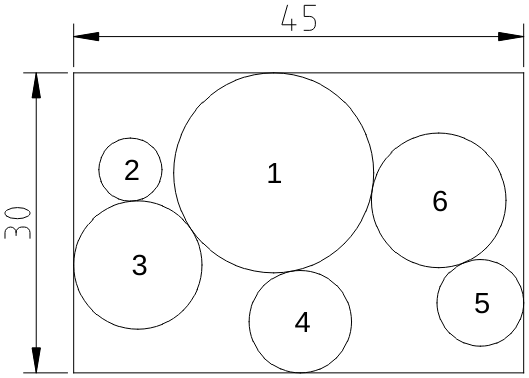
\includegraphics [width=0.4\textwidth]{Bilder/1.png}
 \caption{
 	Darstellung des Problems für $n=6$ Kreise mit zufälliger
 	tangentialer Anordnung der Kreise.
 	Das bemaßte Rechteck stellt die \gls{AABB} für diese Kreisanordnung dar,
 	wobei die Lösung eine Güte von $30 * 45 = 1350$ aufweist.
 	}
 \label{fig:problem_definition}
\end{figure}

\nsecend%{Definition des Problems}


\nsecbegin{Wahl des Genotyps}

Da sich die Kreise im zweidimensionalen reellen Raum bewegen, wurde von einem diskreten Genotyp mit binärer Kodierung abgesehen.
Stattdessen wurden Gleitkommazahlen mit den dazugehörigen, in der Vorlesung vorgestellten, Operatoren verwendet.\\

Die naheliegende Idee, ein Individuum genotypisch durch die Menge der Koordinaten aller Kreismittelpunkte darzustellen, erwies sich schnell als ungeeignet:
Da eine optimale Lösung zwangsläufig tangierende Kreise beinhaltet, sich die Kreise jedoch nicht überlappen dürfen, würde sich ein Optimum stets in größter Nähe einer Vielzahl von ungültigen Individuen befinden. (Siehe Abbildung \ref{fig:wrong_genotype})
Auch würde ein Großteil der möglichen Mutationen ungültige Individuen produzieren, da eine zufällige Bewegung eines Kreises innerhalb einer dichten Anordnung von Kreisen mit hoher Wahrscheinlichkeit zu Kollisionen führt.
Somit wäre ein Optimum sehr schwierig zu finden.\\

\begin{figure}[h]
 \centering
 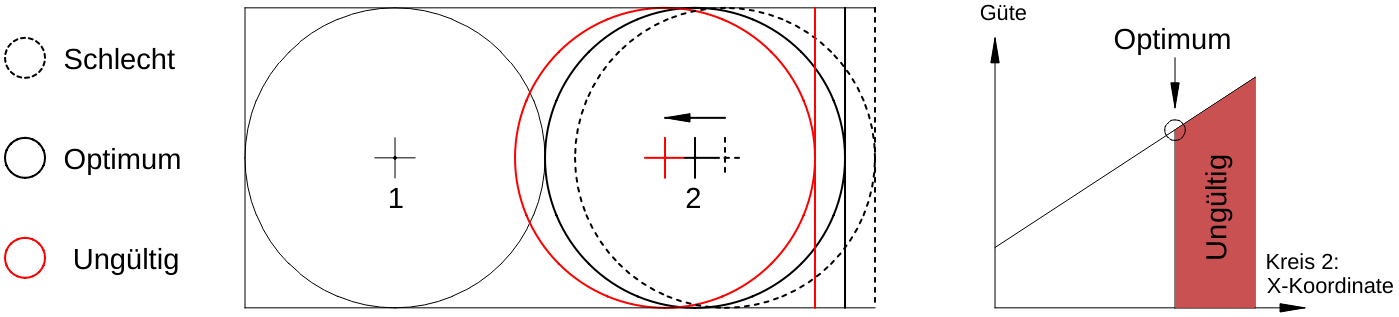
\includegraphics [width=\textwidth]{Bilder/2.png}
 \caption{
 	Vereinfachte Darstellung der Problematik eines koordinatenbasierten
 	Genotyps anhand von n=2 Kreisen.
 	}
 \label{fig:wrong_genotype}
\end{figure}

Eine Implementierung eines deterministischenVerfahrens für genetisches Reparieren erwies sich ebenfalls als schwierig, vermutlich wäre hierfür eine physikalische Kollisionsbehandlung notwendig.\\

In Anlehnung an das in der Vorlesung vorgestellte Beispiel ''Beladen von Containern'' wurde stattdessen ein Dekoder-Ansatz realisiert, welcher ausschließlich gültige Individuen mit tangierenden Kreisen erzeugt.
Da Form und Größe des ''Containers'' - der \gls{AABB} - in der Aufgabenstellung jedoch nicht vorgegeben ist, dient einer der Kreise als Zentrum um welches die anderen Kreise gepackt werden.
Der final gewählte Genotyp besteht aus zwei Teilen, einer Permutation aller n Kreise, sowie einem Kollisionswinkel $a$ ($0 \leq a < 360$) für $n$ Kreise.
(Der Kollisionswinkel des ersten Kreises wird nicht genutzt und ist quasi ''Junk-DNA'', ist jedoch für eine korrekte Mutation der Permutation und für die Rekombination notwendig).\\

Das Dekodieren des Genotyps in eine phänotypische Anordnung wird iterativ durchgeführt:
Initial wird der erste durch die Permutation bestimmte Kreis an der Koordinate $0,0$ im zweidimensionalen reellen Raum positioniert.
Anschließend wird jeder weitere Kreis nacheinander an die bestehenden Kreise angefügt, wobei er sich dem Zentrum in Richtung seines durch den Kollisionswinkel definierten Kollisionsvektors nähert, bis er mit einem der vorhandenen Kreise kollidiert.
Die Koordinate seines Mittelpunktes bei der ersten Kollision entspricht seiner neuen Position, und der nächste Kreis kann analog hierzu angefügt werden, bis allen Kreisen eine Position zugeordnet wurde.
Auf diese Weise können keine ungültigen Individuen entstehen und jedes Individuum ist insofern optimal, dass jeder Kreis mindestens einen weiteren Kreis tangiert.
Ein Beispiel ist in Tabelle \ref{tab:example_genotype} und Abbildung \ref{fig:genotype} dargestellt.\\

\begin{table}[h]
\resizebox{\textwidth}{!}{
\begin{tabular}{|l|l|l|l|l}
\multicolumn{2}{l}{\textit{\textbf{Gegeben}}} & \multicolumn{2}{l}{\textit{\textbf{Genotyp}}}    & \textit{\textbf{Phänotyp}}     \\ \hline
\textbf{n}          & \textbf{Radius}         & \textbf{Permutation} & \textbf{Kollisionswinkel} & \textbf{Dekodierte Koordinate} \\ \hline
1                   & 10                      & 2                    & 225\degree & -15.511452 / 15.601118         \\ \hline
2                   & 12                      & 1                    & X\degree   & 0.0 / 0.0                      \\ \hline
3                   & 7                       & 4                    & 85\degree  & 1.559785 / -18.935867          \\ \hline
4                   & 4                       & 3                    & 188\degree & -21.973601 / 3.181753          \\ \hline
5                   & 15                      & 5                    & 137\degree & -20.439851 / -19.062296        \\ \hline
\end{tabular}
}
\caption{
 	Beispielhafte Darstellung eines Individuums mit $n = 5$ in Genotyp und dekodiertem Phänotyp.
 	}
 \label{tab:example_genotype}
\end{table}

\begin{figure}[h]
 \centering
 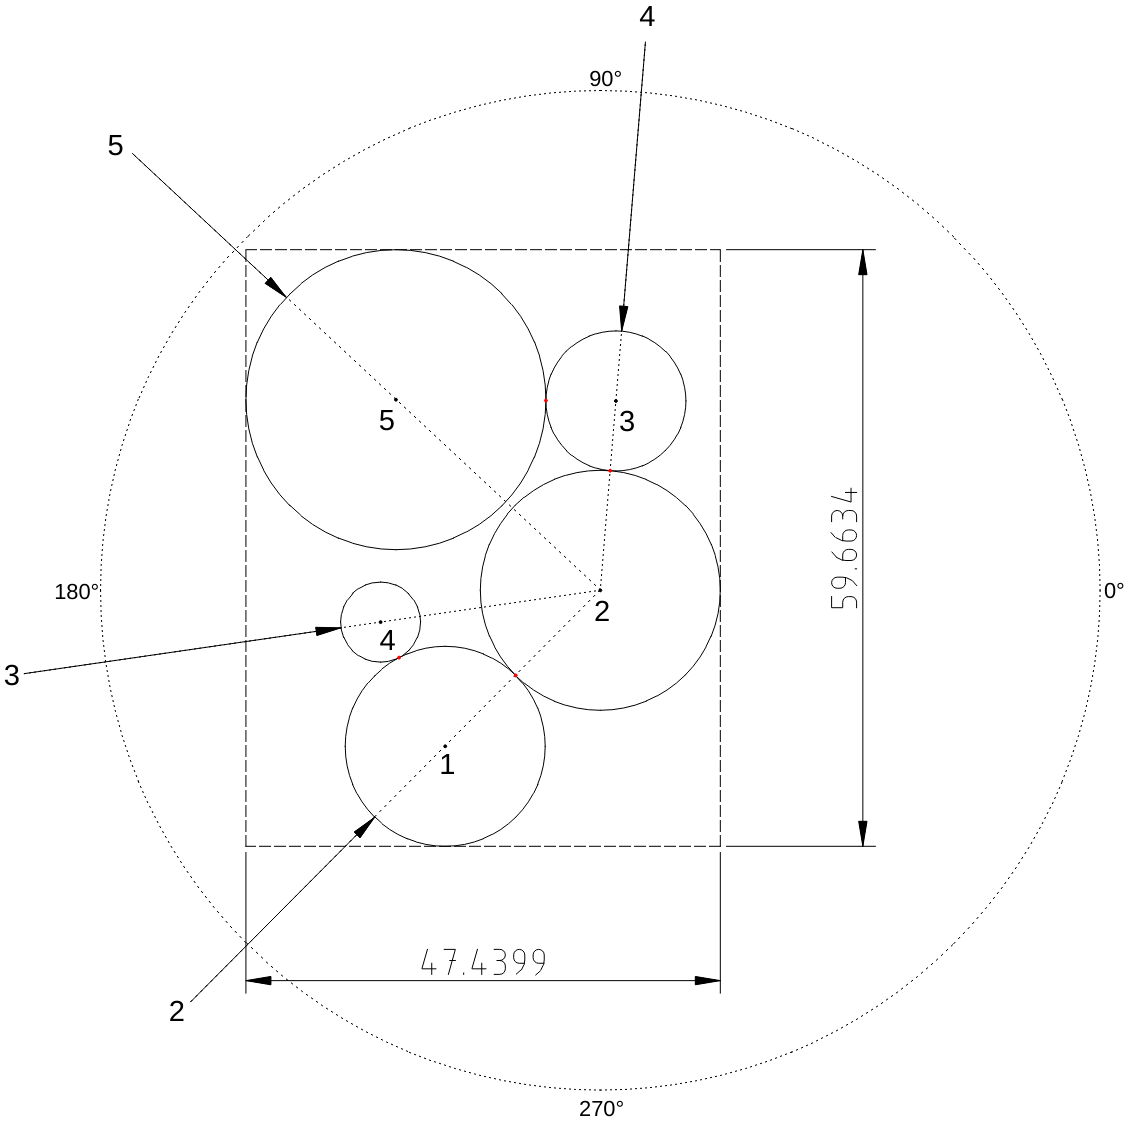
\includegraphics [width=0.75\textwidth]{Bilder/3.png}
 \caption{
 	Visualisierung des Phänotyps von Tabelle \ref{tab:example_genotype}
 	mit angedeuteten Kollisionsvektoren und \gls{AABB}.
 	}
 \label{fig:genotype}
\end{figure}

\nsecend%{Wahl des Genotyps}


\nsecbegin{Wahl der Bewertungsfunktion}

Da der dekodierte Genotyp ausschließlich gültige Individuen erzeugt, kommt die Bewertungsfunktion gänzlich ohne Strafterme aus.
Als zu minimierender Gütewert wird direkt die Fläche der berechneten \gls{AABB} verwendet.\\

Zusätzlich liefert die Bewertungsfunktion die relative Dichte der Lösung als prozentuales Verhältnis zwischen der Gesamtfläche der Kreise und der Fläche der umgebenden \gls{AABB}. Dieser Wert wird jedoch nur im \gls{GUI} angezeigt und wird vom Algorithmus nicht genutzt. Allerdings kann dieser Wert von einem menschlichen Nutzer besser interpretiert werden und erlaubt einen groben Vergleich zwischen Lösungen unterschiedlicher Problemstellungen mit variierender Kreisanzahl oder Kreisdurchmessern.

\nsecend%{Wahl der Bewertungsfunktion}

%%%%%%%%%%%%%%%%%%%%%%%%%%%%%%%%%%%%%%%%%%%%%%%%%%%%%%%%%%%%%%%%%%%%%%%%%%%%%%

\nsecbegin{Ansatz 1 – Lokale Suche}

\nsecbegin{Algorithmus}

Die lokale Suche nutzt eine Populationsgröße von 1 und aus einem Elternidividuum entsteht genau ein Kindindividuum.
Es findet keine Rekombination statt.
Verbesserungen werden immer akzeptiert (Das Kindindividuum ersetzt das Elternindividuum), Verschlechterungen werden nie akzeptiert (Das Elternindividuum bleibt bestehen).
Dies entspricht einem einfachen Hillclimb-Algorithmus, wobei die Mutationsoperatoren und deren Parametrisierung auf den vorliegenden Genotyp angepasst wurden.
Der Algorithmus terminiert nach einer festen, über die \gls{GUI} definierten Anzahl an Generationen, wobei das letzte Individuum dem besten gefundenen entspricht und ausgegeben wird.

\nsecend%{Algorithmus}


\nsecbegin{Mutation der Permutation}

\begin{figure}[h]
 \centering
 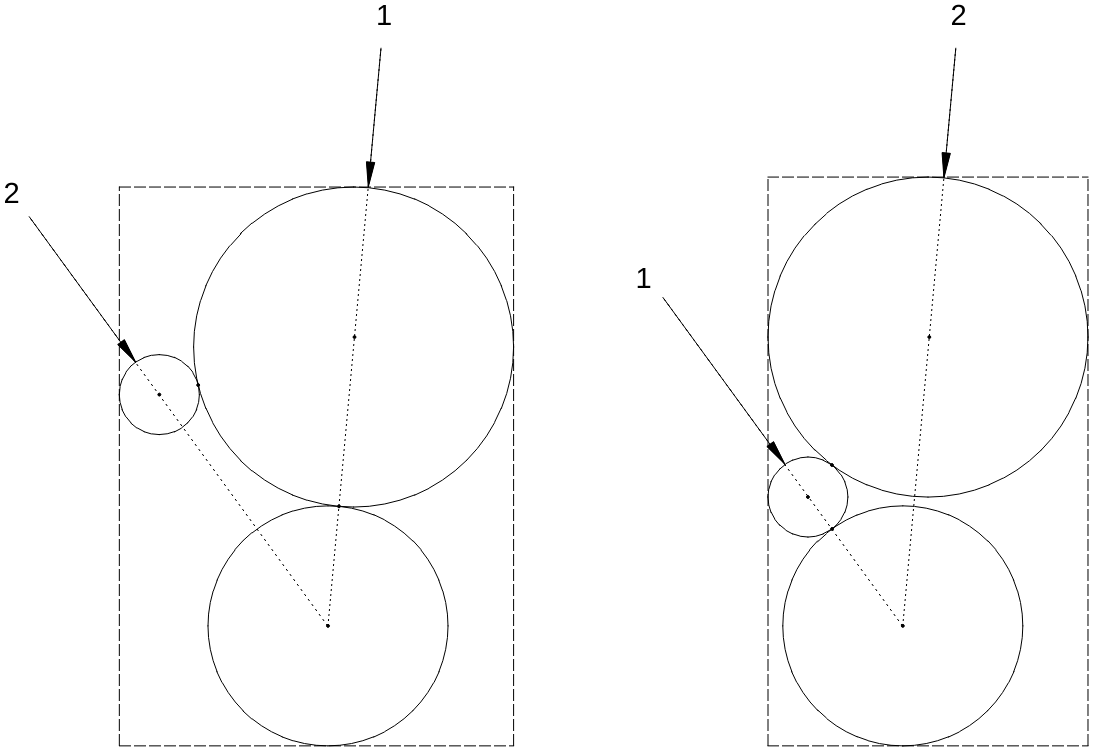
\includegraphics [width=0.7\textwidth]{Bilder/4.png}
 \caption{
 	Beispiel einer vertauschenden Mutation der Permutation eines Individuums,
 	welche zu einer Verbesserung der Güte führt.
 	}
 \label{fig:mutate_permutation_switch}
\end{figure}

Eine Mutation der Permutation der Kreise wird als vertauschende Mutation realisiert.
Dabei wird allein die Reihenfolge in welcher die Kreise angefügt werden verändert, die Winkel und deren Zuordnung zu einzelnen Kreisen bleibt unverändert.
Auf diese Weise können Kreise beispielsweise in Lücken im Inneren der Kreisanordnung hinein rutschen, siehe hierzu Abbildung \ref{fig:mutate_permutation_switch}.\\

Parametrisiert ist diese Mutation durch die Mutationswahrscheinlichkeit pro Kreis.
Im Algorithmus wird über die gesamte Permutation iteriert und jede Position mit der definierten Wahrscheinlichkeit mit einem zufällig gewählten, anderen Kreis vertauscht.

\nsecend %{Mutation der Permutation}


\nsecbegin{Mutation der Winkel}

\begin{figure}[H]
 \centering
 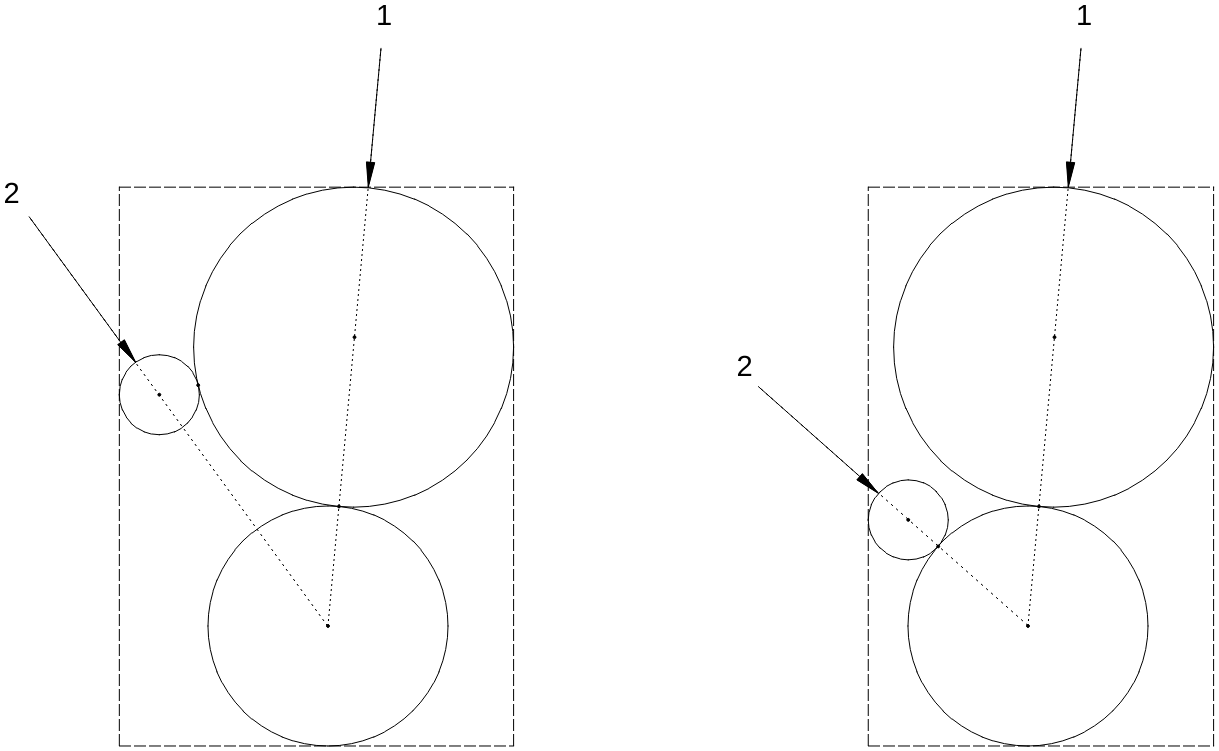
\includegraphics [width=0.78\textwidth]{Bilder/5.png}
 \caption{
 	Beispiel einer Mutation des Kollisionswinkels eines Kreises eines Individuums,
 	welche zu einer Verbesserung der Güte führt.
 	}
 \label{fig:mutate_angle}
\end{figure}

Eine Mutation der Kollisionswinkel der Kreise wird mittels Gauß-Mutation realisiert.
Dabei bleibt die Reihenfolge in welcher die Kreise angefügt werden unverändert.
Durch diese Mutation kann sich die Dichte der Kreise ebenfalls erhöhen, siehe hierzu Abbildung \ref{fig:mutate_angle}.\\

Parametrisiert ist diese Mutation durch die Mutationswahrscheinlichkeit pro Winkel, sowie den Mutationsbereich Sigma, welcher die Standardabweichung der Gaußverteilung definiert.
Im Algorithmus wird über alle Winkel iteriert und jeder mit der definierten Wahrscheinlichkeit innerhalb der Standardabweichung Sigma mutiert.

\nsecend %{Mutation der Winkel}


\nsecbegin{Parametrisierung}

\nsecbegin{Konstant große Mutationen}

Werden die Parameter so gewählt, das während der gesamten Suche sehr große Mutationsschritte verwendet werden, so wird zwar schnell eine mittelmäßige Lösung erreicht, doch mangelt es anschließend an der Feinabstimmung um die Anordung weiter zu optimieren.
Im Beispiel aus Abbildung \ref{fig:hillclimb_constbig} wurde die Mutationswahrscheinlichkeit der Permutation konstant auf $\frac{1}{5}$ gesetzt, die Mutationswahrscheinlichkeit der Winkel konstant auf $\frac{1}{4}$ und die Standardabweichung Sigma für die Größe der Winkelmutation auf $90\degree$ festgelegt.
Das Problem wurde zufällig mit $n = 40$ Kreisen initialisiert und über $100.000$ Generationen hinweg optimiert.
Im Mittel über 10 Durchläufe wurde eine relative Dichte von $58,32\%$ ermittelt.

\begin{figure}[h]
 \centering
 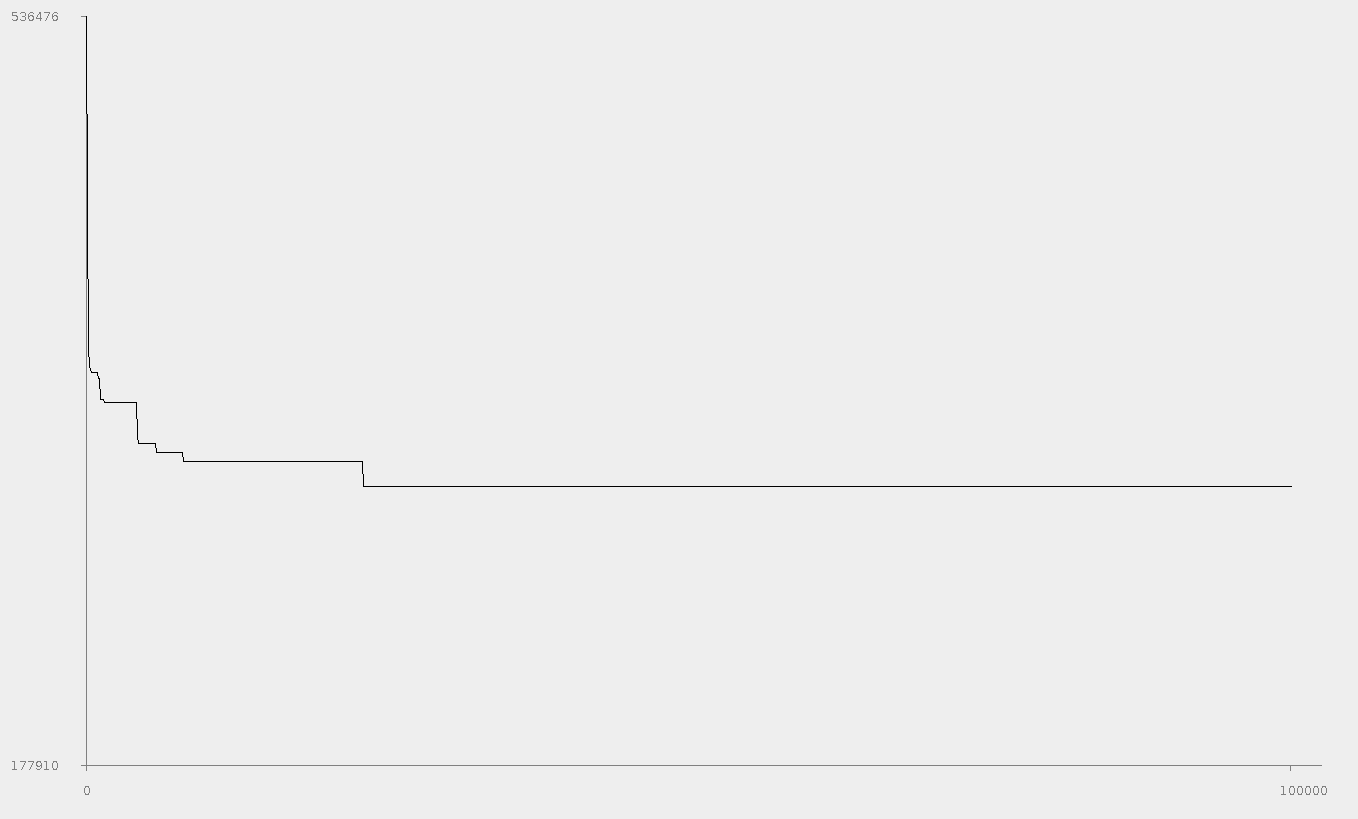
\includegraphics [width=0.6\textwidth]{Bilder/Hillclimb_constbig.png}
 \caption{
 	Zeitreihe einer lokalen Suche über $100.000$ Generationen mit $n = 40$
 	und konstant großen Mutationsschritten.
 	}
 \label{fig:hillclimb_constbig}
\end{figure}

\nsecend%{Konstant große Mutationen}


\nsecbegin{Konstant kleine Mutationen}

Werden die Parameter so gewählt, das während der gesamten Suche sehr kleine Mutationsschritte verwendet werden, so wird die bestehende Anordnung zwar fein optimiert, jedoch wird der gesamte Suchraum nicht ausreichend erforscht und der Algorithmus endet in einem lokalen Optimum.
Im Beispiel aus Abbildung \ref{fig:hillclimb_constsmall} wurde die Mutationswahrscheinlichkeit der Permutation konstant auf $\frac{1}{n}$ gesetzt, die Mutationswahrscheinlichkeit der Winkel konstant auf $\frac{1}{n}$ und die Standardabweichung Sigma für die Größe der Winkelmutation auf $5\degree$ festgelegt.
Das Problem wurde zufällig mit $n = 40$ Kreisen initialisiert und über $100.000$ Generationen hinweg optimiert.
Im Mittel über 10 Durchläufe wurde eine relative Dichte von $73,93\%$ ermittelt.

\begin{figure}[h]
 \centering
 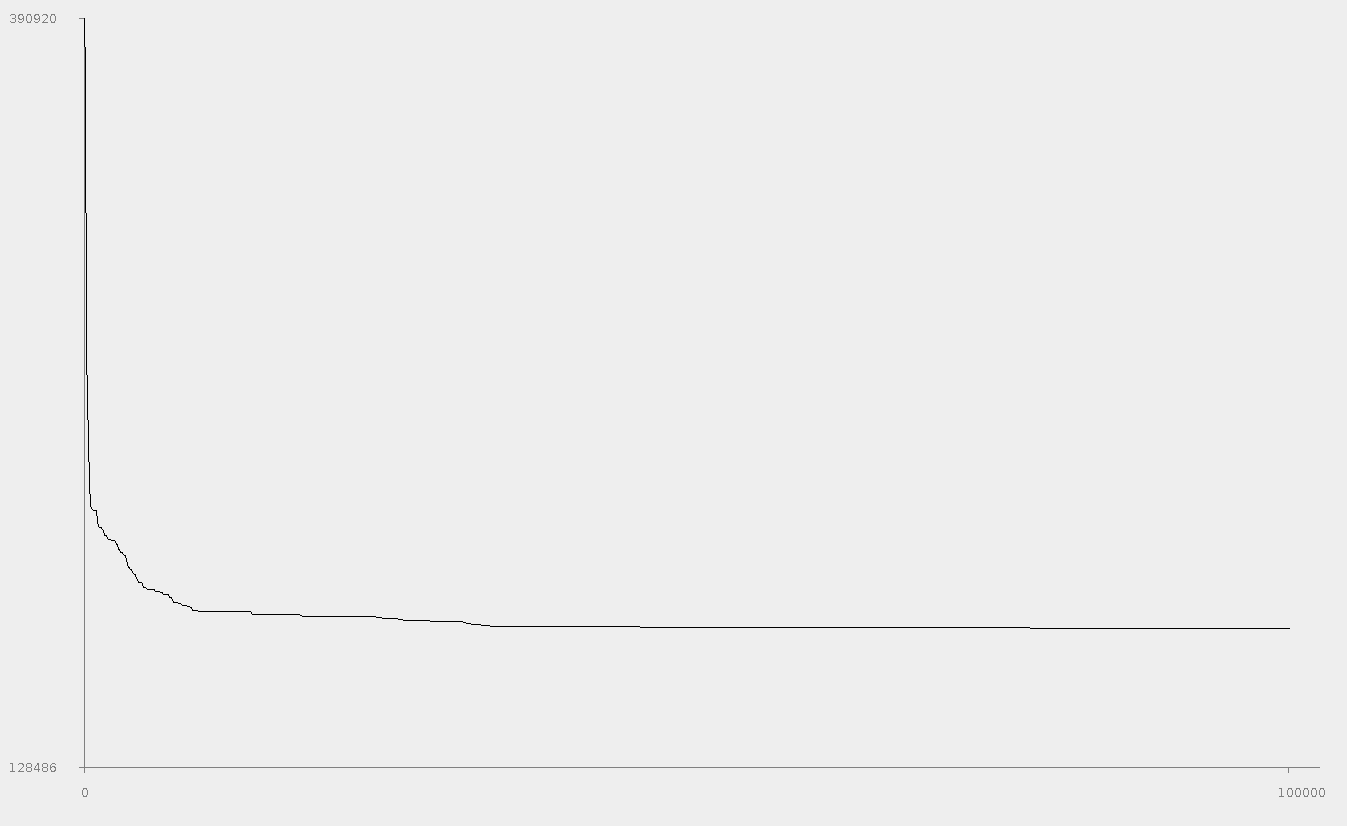
\includegraphics [width=0.6\textwidth]{Bilder/Hillclimb_constsmall.png}
 \caption{
 	Zeitreihe einer lokalen Suche über $100.000$ Generationen mit $n = 40$
 	und konstant kleinen Mutationsschritten.
 	}
 \label{fig:hillclimb_constsmall}
\end{figure}

\nsecend%{Konstant kleine Mutationen}


\nsecbegin{Variable Mutationsraten}

In der finalen Implementierung sind die Mutationsraten variabel gewählt und werden automatisch zur Laufzeit berechnet.
Die Idee besteht darin, zu Beginn der lokalen Suche mit großen Mutationsschritten zu arbeiten um den Suchraum weiträumig zu erkunden, während zum Ende der Suche mit sehr kleinen Mutationsschritten gearbeitet wird, um die bestehende Anordnung in der Feinabstimmung zu optimieren.\\

Der Algorithmus zur Berechnung der Parameter wurde empirisch entwickelt und iterativ optimiert.
Das Grundprinzip besteht darin, einen initialen Wert in jeder Generation mit einem Dämpfungsfaktor $d$ mit $0.9 < d < 1$ zu multiplizieren.
Zu Beginn der Optimierung wird der initiale Wert und der Dämpfungsfaktor $d$ auf Basis von $n$ und der Anzahl an Generationen ermittelt.
Die Parameter werden wie folgt ermittelt:\\

Die Mutationswahrscheinlichkeit der Permutation liegt zu Beginn der Optimierung bei $\frac{1}{4}$ und schrumpft bis zur Halbzeit der Suche (Hälfte der vorgesehenen Generationen) auf $\frac{1}{n}$. In der zweiten Hälfte der Suche schrumpft die Mutationswahrscheinlichkeit der Permutation konstant weiter und ist dann $<\frac{1}{n}$ womit die Mutation der Permutation für die zweite Hälfte der Optimierung nur eine untergeordnete Rolle spielt.\\

Die Mutationswahrscheinlichkeit der Winkel wird konstant auf $\frac{4}{n}$ festgelegt, die Verkleinerung der Mutationsschritte erfolgt allein über den variablen Wert der Standardabweichung Sigma.\\

Die Standardabweichung Sigma wird initial auf $180\degree$ festgelegt und schrumpft bis zum Ende der Suche auf $1\degree$.\\

Im Beispiel aus Abbildung \ref{fig:hillclimb_variabel} wurde wieder ein Problem zufällig mit $n = 40$ Kreisen initialisiert und über $100.000$ Generationen hinweg optimiert.
Im Mittel über 10 Durchläufe wurde eine relative Dichte von $75,22\%$ ermittelt, wobei der Bereich in welchem sich die Werte bewegen weiterhin sehr groß geblieben ist ($69.42\% - 78,81\%$).

\begin{figure}[h]
 \centering
 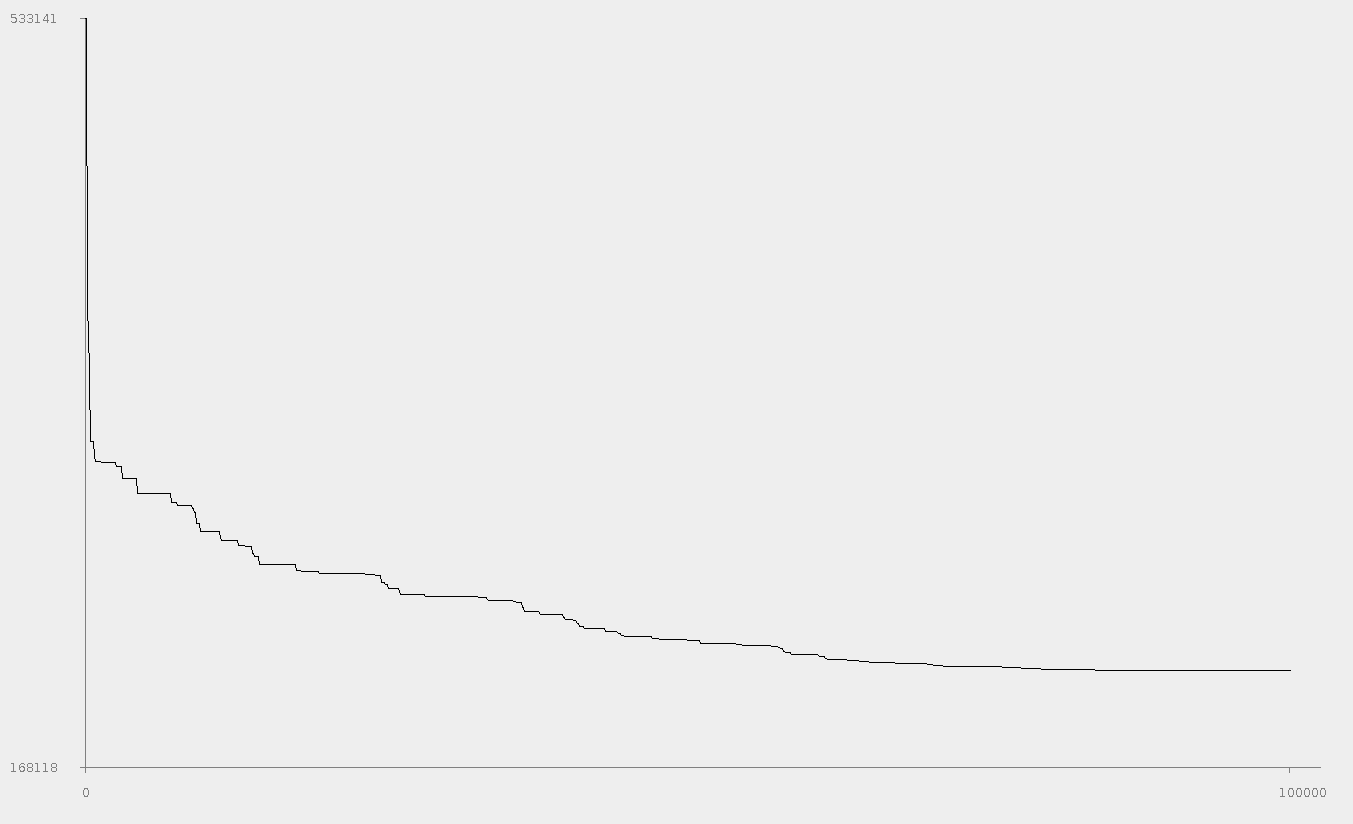
\includegraphics [width=0.6\textwidth]{Bilder/Hillclimb_variable.png}
 \caption{
 	Zeitreihe einer lokalen Suche über $100.000$ Generationen mit $n = 40$ und variabler Mutationsschrittweite.
 	}
 \label{fig:hillclimb_variabel}
\end{figure}

\nsecend%{Variable Mutationsraten}

\nsecend%{Parametrisierung}

\nsecend %{Ansatz 1 – Lokale Suche}

%%%%%%%%%%%%%%%%%%%%%%%%%%%%%%%%%%%%%%%%%%%%%%%%%%%%%%%%%%%%%%%%%%%%%%%%%%%%%%

\nsecbegin{Ansatz 2 - Genetischer Algorithmus}

\nsecbegin{Algorithmus}

Beim genetischen Algorithmus existiert eine Elternpopulation aus welcher in jeder Generation eine Kindpopulation erzeugt wird, welche die Elternpopulation in der nächsten Generation ersetzt.
Die Populationsgröße kann über die \gls{GUI} eingestellt werden.
Die Größe der Elternpopulation ist identisch mit der Größe der Kindpopulation.
Kindindividuen werden durch Rekombination zweier Elternindividuen erzeugt.
Der Selektionsdruck ist in Form einer Turnierselektion bei der Auswahl der Elternindividuen realisiert, wobei die Anzahl an Gegner-Individuen pro Turnierrunde als $\frac{n}{8}+1$ festgelegt ist.
Die versuchsweise Implementierung einer rangbasierten Elternselektion erwies sich gegenüber der Turnierselektion als suboptimal.

\nsecend%{Algorithmus}


\nsecbegin{Rekombination}

Die Kombination zweier Elternindividuen zu einem Kindindividuum erwies sich als ausgesprochen schwierig.
Die Rekombination der Permutation wurde als Ordnungsrekombination realisiert, da die Reihenfolge hier die relevante Eigenschaft der Permutation ist.
Die Zuordung der Kollisionswinkel zu Kreisen bleibt bestehen, da die Ordnungsrekombination implizit auch für die Kollisionswinkel durchgeführt wird.\\

Ein erster Ansatz wurde als Variante des 1-punkt-Crossovers realisiert.
Ein zufälliger Schnittpunkt $s$ mit $0 < s < n$ wird als Trennstelle gewählt, wobei der erste Bereich aus dem ersten Elternindividuum übernommen wird und der zweite Bereich gemäß der Ordnungsrekombination mit den verbleibenden Werten aus dem zweiten Elternindividuum aufgefüllt wird.
Leider hat sich gezeigt das zwei zufällige Hälften zweier Elternindividuen nur selten gut ''zusammen passen'' und ein Kindindividuum fast immer schlechter als seine Eltern bewertet wird.\\

Im zweiten und finalen Ansatz wurde versuchst, die räumliche Nähe der Kreise innerhalb der Elternindividuen stärker zu berücksichtigen.
Es wird ein Bereich von Kollisionswinkeln zufällig gewählt, welcher als Auswahlkriterium für die Übernahme eines Kreises aus dem ersten Elternindividuum fungiert.
Alle Kreise dessen Kollisiosnswinkel innerhalb des gewählten Bereichs liegen, werden aus dem ersten Elternindividuum übernommen, alle weiteren werden gemäß der Ordnungsrekombination aus dem zweiten Elternindividuum aufgefüllt.
Dies kann als Variation des k-punkt-Crossovers aufgefasst werden.
Zwar bleibt so ein räumlich zusammen passender Bereich des ersten Elternindividuums bestehn, doch da aus dem zweiten Elternindividuum weiterhin alle fehlenden Kreise ungeachtet ihrer Anordnung übernommen werden müssen, passen die beiden Hälften der Elternindividuen nach wie vor schlecht zusammen. Der Effekt ist bei disem Ansatz geringer als beim ersten Versuch, jedoch sind Kindindividuen weiterhin meist schlechter als ihre Elternindividuen.

\nsecend%{Rekombination}

\nsecbegin{Mutationsoperatoren}

Die Mutationsoperatoren sind identisch zu denen der lokalen Suche realisiert. Die versuchsweise Implementierung einer verschiebenden Mutation der Permutation erwies sich gegenüber der vertauschenden Mutation als ungeeignet.

\nsecend%{Mutationsoperatoren}


\nsecbegin{Parametrisierung}

Die Parametrisierung der Mutationsoperatoren wurde durch mehrere Versuche empirisch ermittelt und wurde final wie folgt festgelegt:\\

Die Mutationswahrscheinlichkeit der Permutation ist variabel und liegt zu Beginn der Optimierung bei $\frac{2}{n}$, wobei sie bis zum Ende der Suche auf $\frac{1}{2n}$ sinkt.\\

Die Mutationswahrscheinlichkeit der Winkel ist konstant auf $0.25$ festgelegt, sodass im Mittel ein Viertel aller Kollisionswinkel mutiert wird.\\

Die Standardabweichung Sigma der Gaußmutation der Kollisionswinkel wird initial auf $240\degree$ festgelegt und schrumpft bis zum Ende der Suche auf $2\degree$.

\begin{figure}[H]
 \centering
 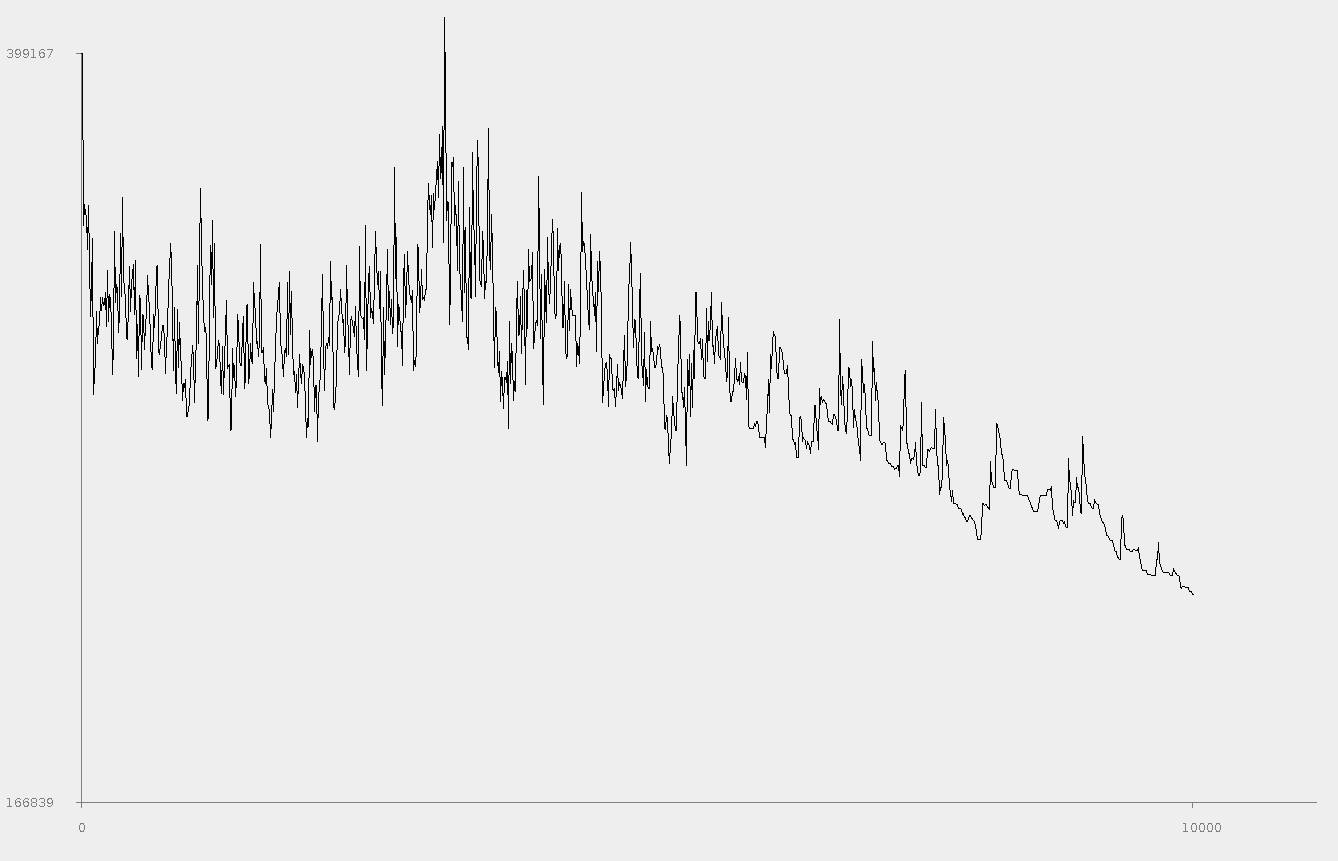
\includegraphics [width=0.6\textwidth]{Bilder/Genetic_20.png}
 \caption{
 	Zeitreihe einer genetischen Suche über $10.000$ Generationen mit Populationsgröße $20$ und $n = 40$.
 	Die Ergebnisse sind stark schwankend, über 10 Durchläufe wurden im Mittel nur 69,81\% relative Dichte erreicht.
 	}
 \label{fig:genetic_20}
\end{figure}

\begin{figure}[H]
 \centering
 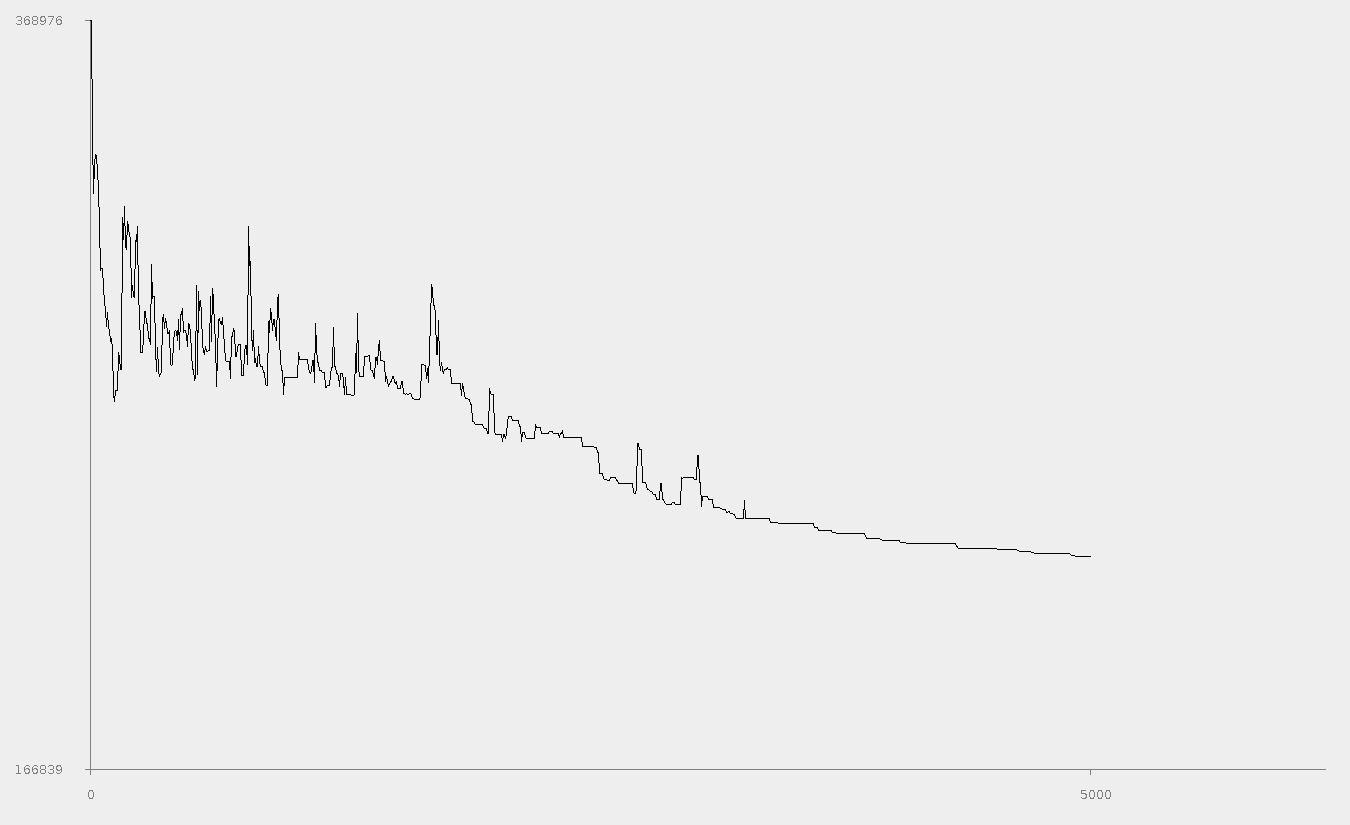
\includegraphics [width=0.6\textwidth]{Bilder/Genetic_40.png}
 \caption{
 	Zeitreihe einer genetischen Suche über $5.000$ Generationen mit Populationsgröße $40$ und $n = 40$.
 	Über 10 Durchläufe wurde im Mittel eine relative Dichte von 74,66\% ermittelt,
 	wobei die Ergebnisse recht stabil in diesem Bereich liegen (ca. $+/- 1\%$).
 	}
 \label{fig:genetic_40}
\end{figure}

\begin{figure}[H]
 \centering
 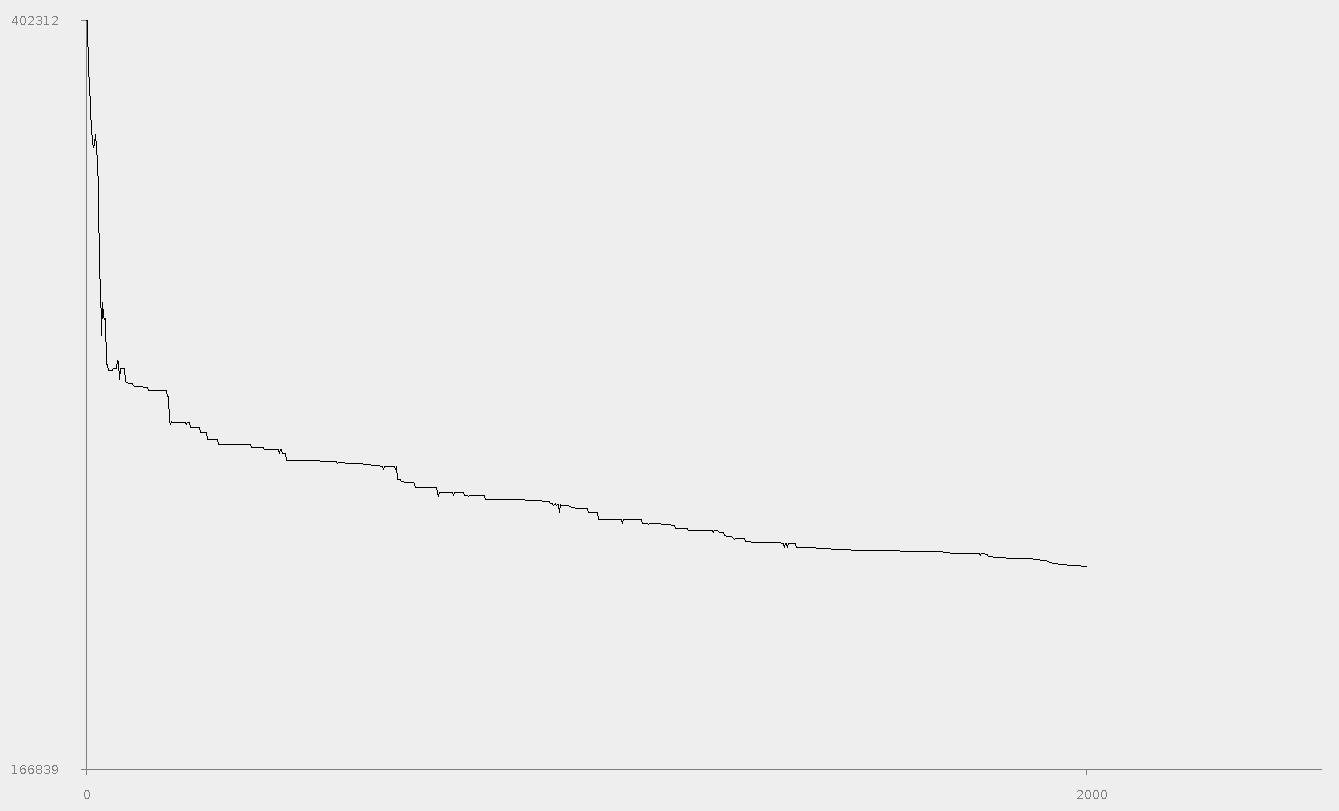
\includegraphics [width=0.6\textwidth]{Bilder/Genetic_100.png}
 \caption{
 	Zeitreihe einer genetischen Suche über $2.000$ Generationen mit Populationsgröße $100$ und $n = 40$.
 	Über 10 Durchläufe wurde im Mittel eine relative Dichte von 71,93\%, wobei die Schwankungen
 	der finalen Güte über mehrere Durchläufe wieder verstärkt schwanken.
 	}
 \label{fig:genetic_100}
\end{figure}

Die Populationsgröße ist über die \gls{GUI} frei einstellbar, empirische Untersuchungen ergaben jedoch das sich eine optimale Populationsgröße im Bereich $40-50$ liegt. Für die Studie wurde ein Problem mit $n = 40$ und insgesamt $200.000$ Auswertungen (Populationsgröße * Anzahl der Generationen) betrachtet. Die Ergebnisse sind in Abbildung \ref{fig:genetic_20} bis \ref{fig:genetic_100} dargestellt, wobei die Zeitreihe für jede Generation das beste Individuum anzeigt. Wie sich gezeigt hat erreicht der genetische Algorithmus selbst bei scheinbar optimaler Parametrisierung nicht die Güte der lokalen Suche, obwohl in den Versuchsreihen für ein identisches Problem bereits die doppelte Menge an Auswertungen ausgeführt wurde. Bemerkenswert ist jedoch, dass die Güte des finalen Ergebnisses über mehrere Durchläufe beim genetischen Algorithmus viel stabiler ist als bei der lokalen Suche und nur in einem kleinen Bereich von wenigen Prozentpunkten variiert.

\nsecend%{Parametrisierung}

\nsecend%{Ansatz 2 - Genetischer Algorithmus}

%%%%%%%%%%%%%%%%%%%%%%%%%%%%%%%%%%%%%%%%%%%%%%%%%%%%%%%%%%%%%%%%%%%%%%%%%%%%%%

\nsecbegin{Ansatz 3 - Evolutionsstrategie}

\nsecbegin{Algorithmus}

Da sich die Rekombination als Schwachstelle des genetischen Algorithmus gezeigt hat, wurde im dritten Ansatz eine Evolutionsstrategie entwickelt.
Hierbei existiert ebenfalls eine Elternpopulation, aus welcher mittels einfacher Mutationsoperatoren (ohne Rekombination) eine Kindpopulation erzeugt wird, wobei ein Vielfaches der Populationsgröße $p$ an Kindern erzeugt wird.
Das Vielfache ist über die Reproduktionsrate $r$ definiert.
Aus den $p * r$ Kindindividuen werden die besten $p$ Individuen in die neue Elterngeneration übernommen (''Komma''-Strategie) bzw. die besten $p$ Individuen aus Kind- und Elterngeneration werden in die neue Elterngeneration übernommen (''Plus''-Strategie).\\

In der klassischen Variante der Evolutionsstrategie werden die Elternindividuen zur Erzeugung der Kindindividuen uniform aus der Population gewählt, der Selektionsdruck ist allein durch die Übernahme der besten $p$ Individuen gegeben.
Es hat sich jedoch gezeigt das der Algorithmus für das vorliegende Problem bessere Ergebnisse erzielt, wenn der Selektionsdruck zusätzlich durch eine Elternselektion erhöht wird.
In der Implementierung kommt ebenfalls die Turnierselektion zum Einsatz.\\

\nsecend%{Algorithmus}

\nsecbegin{Parametrisierung}

Ursprünglich sollte die Evolutionsstrategie mit selbstadaptiver Schrittweitenanpassung zur Einstellung der Standardabweichung Sigma der Winkelmutation, sowie ggf. der Einstellung der Mutationswahrscheinlichkeiten, arbeiten.
Leider hat dieser Ansatz dazu geführt das die Schrittweiten bzw. Mutationswahrscheinlichkeiten bereits nach wenigen Generation zu $0$ konvergieren.
Vermutlich weil kleine Schrittweiten bei dem vorliegenden Problem mit höherer Wahrscheinlichkeit zu einer Verbesserung führen und damit in die nächste Generation übernommen werden, auch wenn die Verbesserungen in diesem Fall marginal sind.\\

Die Mutationsoperatoren sind in der finalen Implementierung identisch zu denen der lokalen Suche parametrisiert.
Hinzugekommen sind Populationsgröße und Reproduktionsrate als zusätzliche Parameter, welche über die \gls{GUI} einstellbar sind.
Außerdem kann zwischen ''Komma''- und ''Plus''-Strategie gewählt werden.\\

Die Zeitreihen für ''Komma''- und ''Plus''-Strategie unterscheiden sich optisch deutlich (Siehe Abbildungen \ref{fig:strategy_komma_40_5} und \ref{fig:strategy_plus_40_5}), da es nur bei der Komma-Strategie zu Verschlechterungen kommen kann.
Die Ergebnisse fallen jedoch sehr ähnlich aus. Ein Überblick über durchschnittliche Gütewerte bei variierender Populationsgröße und Reproduktionsrate ist in Tabelle \ref{tab:strategy_params} gegeben.\\

Insgesamt scheint die Evolutionsstrategie die besten Ergebnisse zu liefern, wenn die Reproduktionsrate eher gering ist, im Bereich $3 - 8$.
Eine hohe Populationsgröße scheint zu einer höheren Stabilität der Ergebnisse zu führen, auch wenn eine niedrige Populationsgröße im Mittel bessere Ergebnisse erzielt, insbesondere bei Anwendung der ''Komma''-Strategie.

\begin{figure}[H]
 \centering
 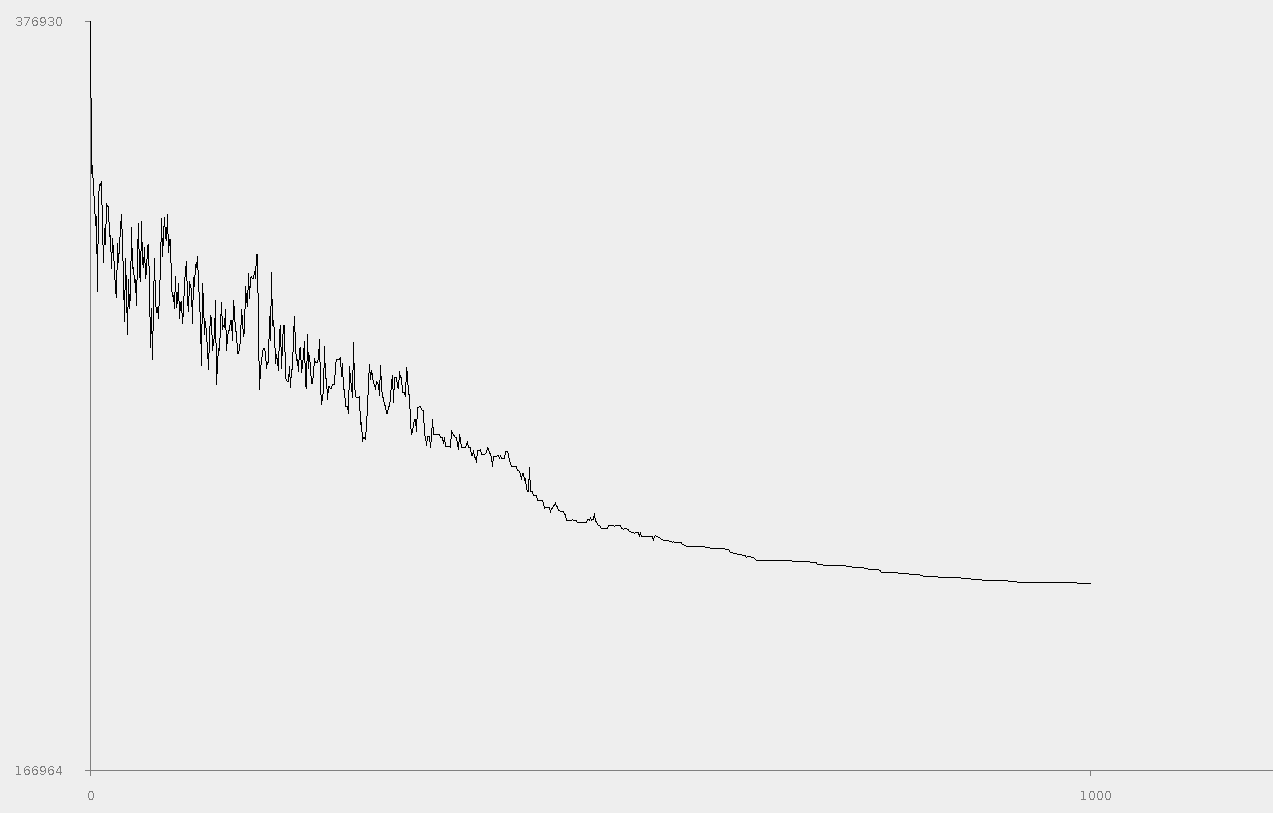
\includegraphics [width=0.6\textwidth]{Bilder/Strategy_komma_40_5.png}
 \caption{
 	Zeitreihe einer Evolutionsstrategie (''Komma''-Strategie) über $1.000$ Generationen mit Populationsgröße $40$,
 	Reproduktionsrate $5$ und $n = 40$.
 	Über 10 Durchläufe wurden im Mittel 76,04\% relative Dichte erreicht,
 	die Ergenbnisse schwanken um ca. $+/- 2\%$.
 	}
 \label{fig:strategy_komma_40_5}
\end{figure}
 
\begin{figure}[H]
 \centering
 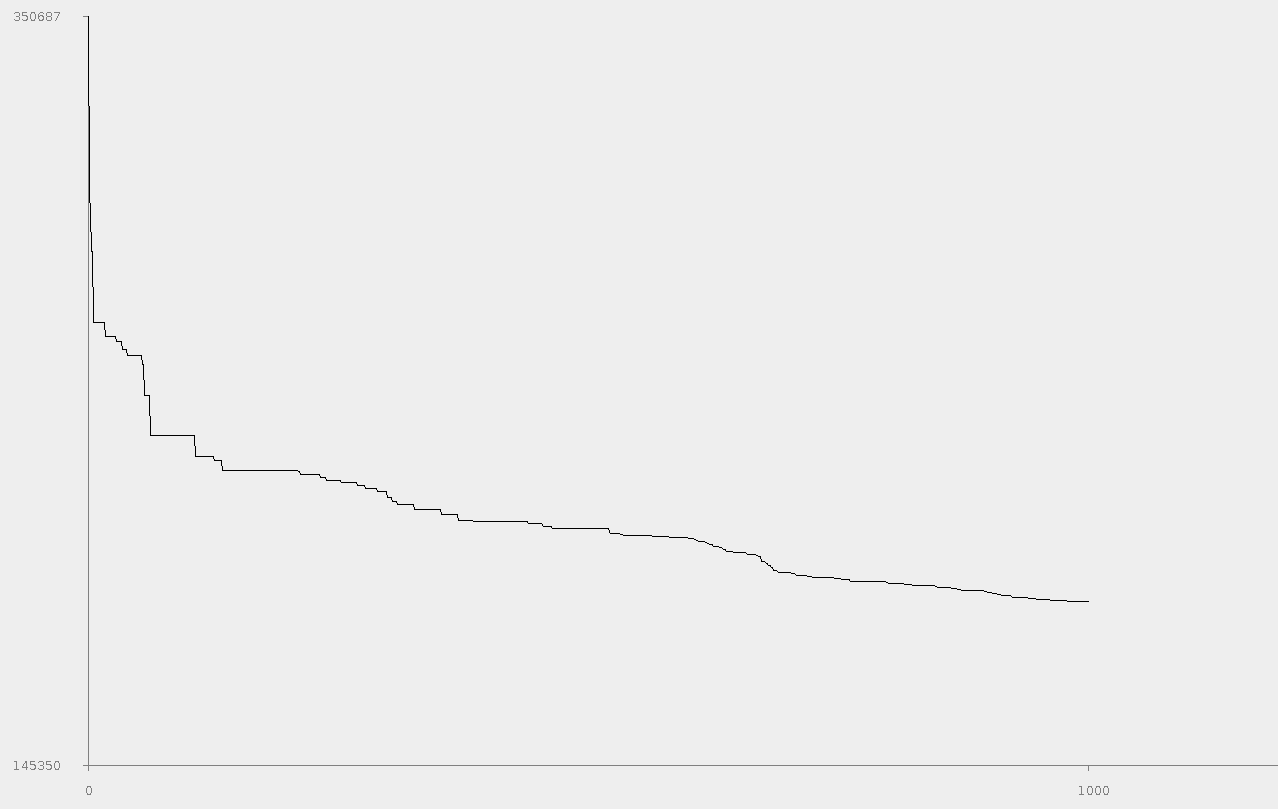
\includegraphics [width=0.6\textwidth]{Bilder/Strategy_plus_40_5.png}
 \caption{
 	Zeitreihe einer Evolutionsstrategie (''Plus''-Strategie) über $1.000$ Generationen mit Populationsgröße $40$,
 	Reproduktionsrate $5$ und $n = 40$.
 	Über 10 Durchläufe wurden im Mittel 76,19\% relative Dichte erreicht,
 	die Ergenbnisse schwanken um ca. $+/- 1\%$.
 	}
 \label{fig:strategy_plus_40_5}
\end{figure}

\begin{table}[]
\resizebox{\textwidth}{!}{
\begin{tabular}{|l|l|l|l|l|l|}
\hline
\textbf{Strategie} & \textbf{Generationen} & \textbf{Populationsgröße} & \textbf{Reproduktionsrate} & \textbf{Mittlere Güte} & \textbf{Geschätzte Abweichung} \\ \hline
Komma              & 1.000                 & 40                        & 5                          & 76,04\%                & $+/- 2\%$        \\ \hline
Plus               & 1.000                 & 40                        & 5                          & 76,19\%                & $+/- 1\%$        \\ \hline
Komma              & 1.000                 & 10                        & 20                         & 75,49\%                & $+/- 2\%$        \\ \hline
Plus               & 1.000                 & 10                        & 20                         & 75,72\%                & $+/- 1.5\%$      \\ \hline
Komma              & 10.000                & 5                         & 4                          & 76,81\%                & $+/- 2.5\%$      \\ \hline
Plus               & 10.000                & 5                         & 4                          & 74,90\%                & $+/- 3\%$        \\ \hline    
\end{tabular}%
}
\caption{
 	Auswertung der Evolutionsstrategie mit unterschiedlichen Werten für Populationsgröße $p$ und Reproduktionsrate $r$ über jeweils $200.000$ Auswertungen. Die Mittlere Güte wurde jeweils über 10 Durchläufe ermittelt.
 	}
 \label{tab:strategy_params}
\end{table}

\nsecend%{Parametrisierung}

\nsecend%{Ansatz 3 - Evolutionsstrategie}

%%%%%%%%%%%%%%%%%%%%%%%%%%%%%%%%%%%%%%%%%%%%%%%%%%%%%%%%%%%%%%%%%%%%%%%%%%%%%%

\nsecbegin{Auswertung der finalen Implementierungen}

\nsecbegin{Benchmark-Test}

Da für das vorliegende Problem keine vorgefertigten Benchmark-Datensätze ausfindig gemacht werden konnten, wurde ein Benchmarktest mit bekanntem Optimum eigens entwickelt. Die offensichtlich optimale Anordnung und die dazugehörigen Kreisradien sind in Abbildung \ref{fig:benchmark} dargestellt.\\

\begin{figure}[h]
 \centering
 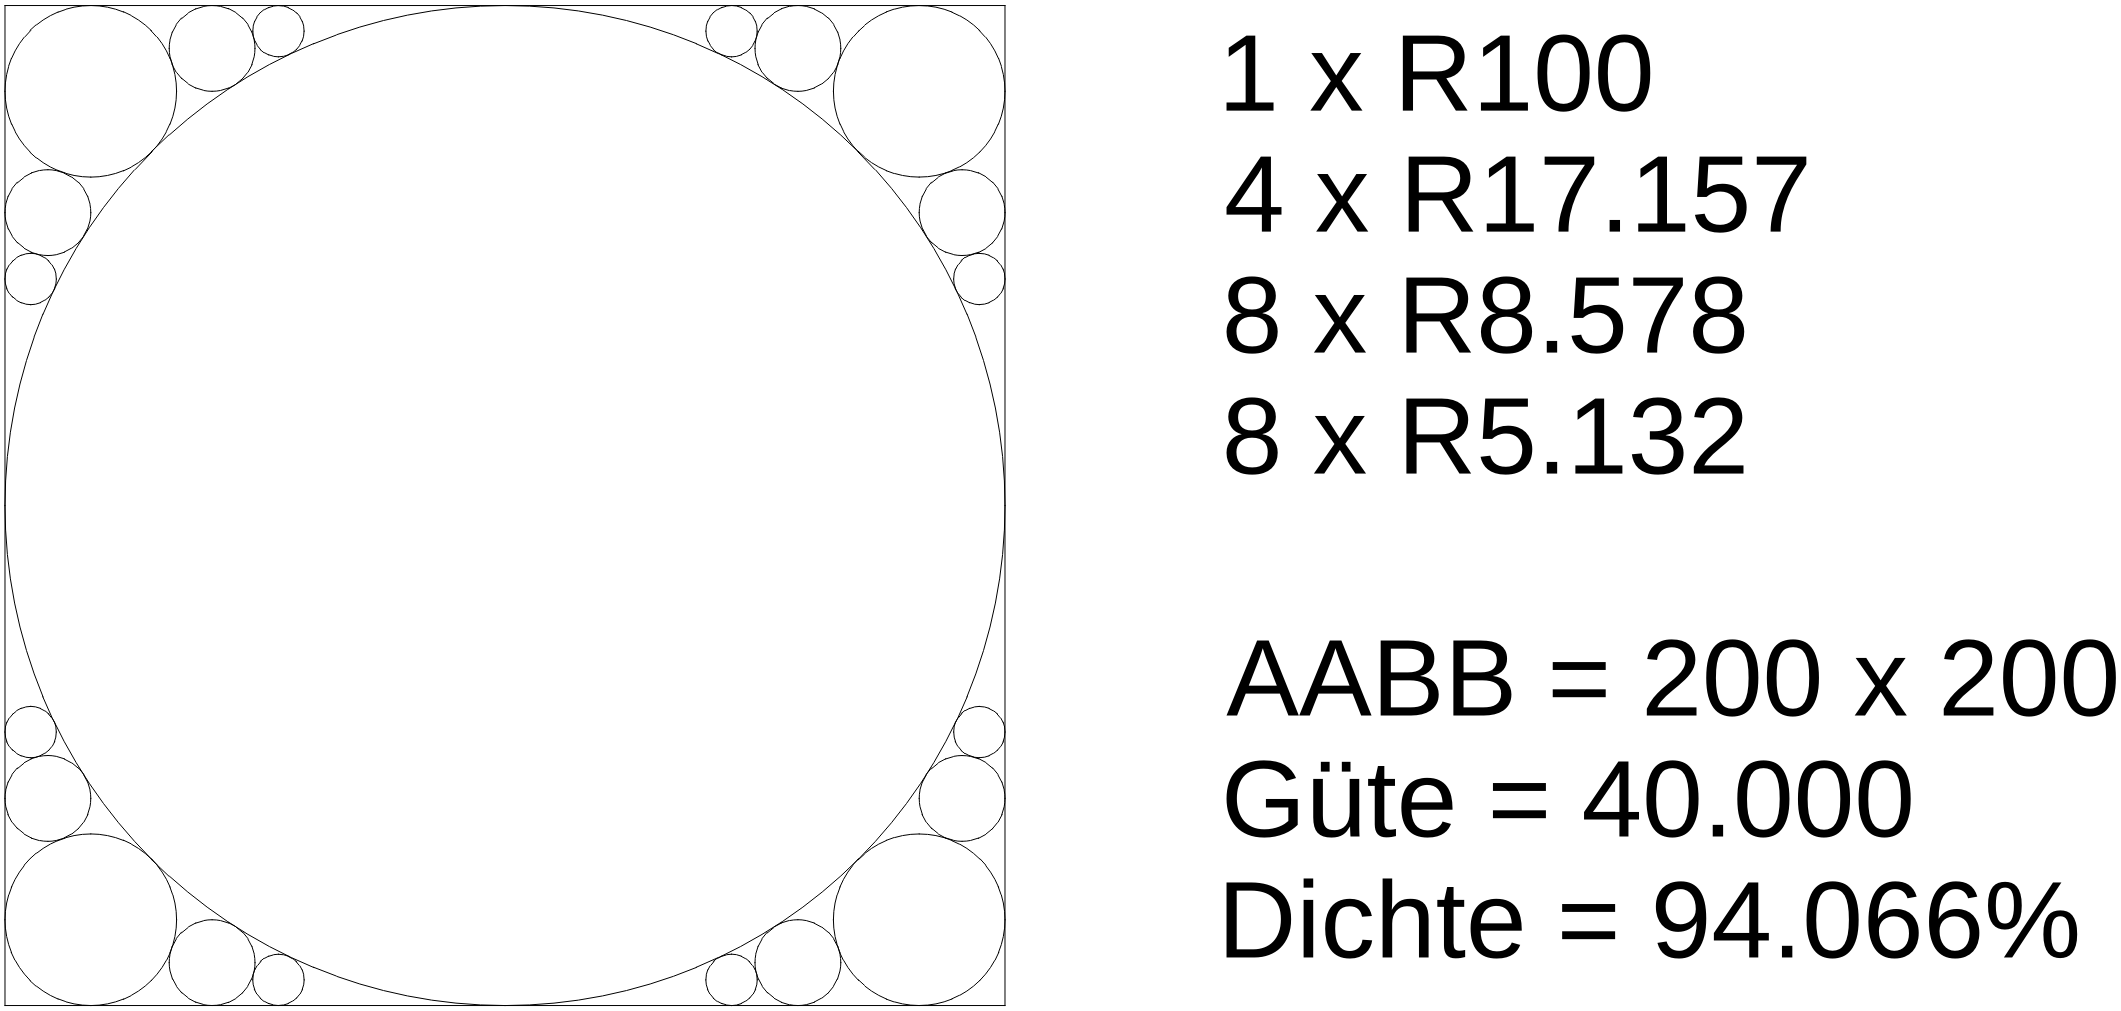
\includegraphics [width=0.8\textwidth]{Bilder/6.png}
 \caption{
 	Gewähltes Benchmark-Problem mit $n = 21$ und Optimum bei $40.000$ bzw. einer Dichte von $94,066\%$.
 	}
 \label{fig:benchmark}
\end{figure}

\begin{figure}[h]
 \centering
 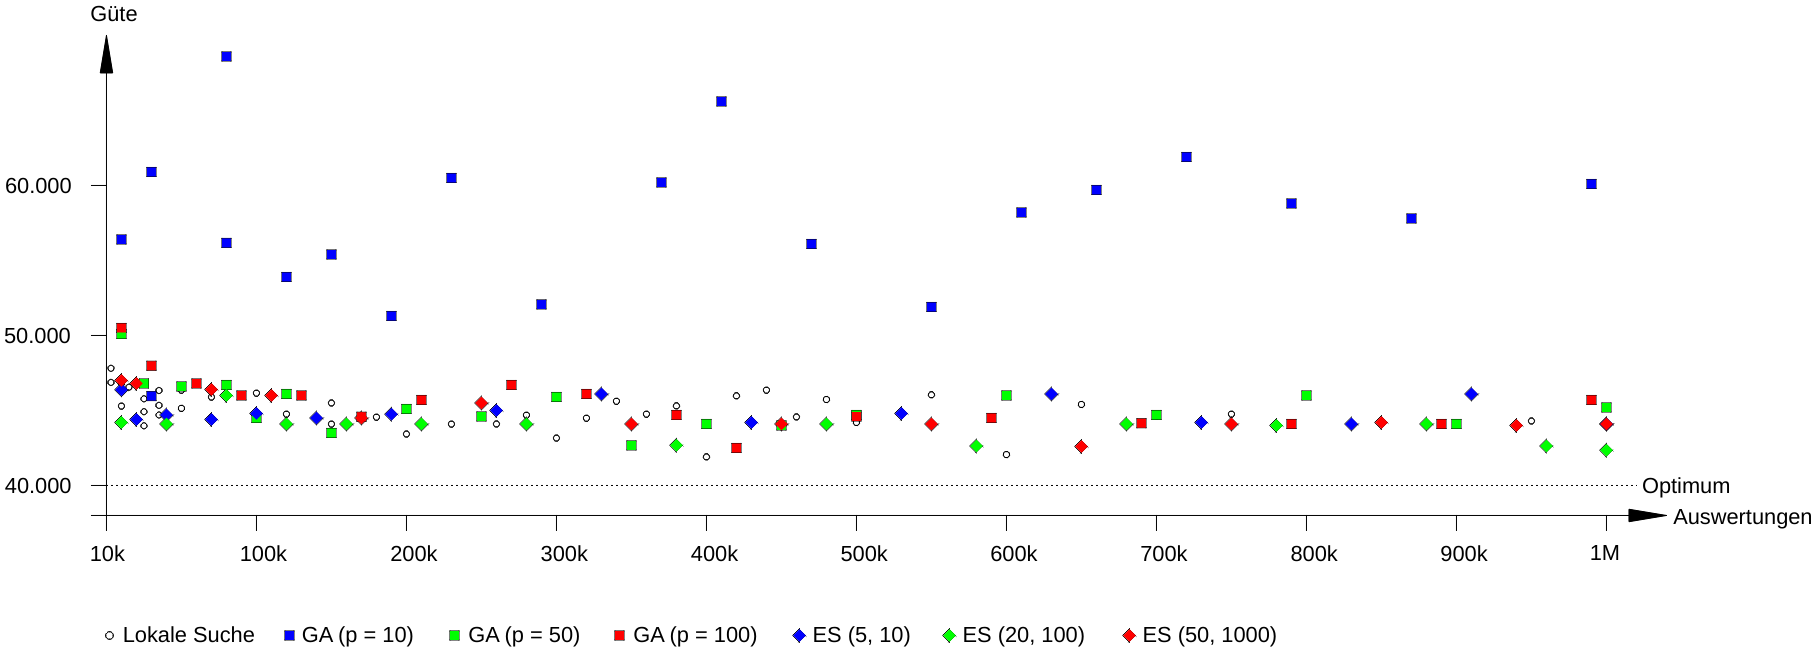
\includegraphics [width=1\textwidth]{Bilder/benchmark.png}
 \caption{
 	Auswertung des Benchmark-Problems mit $n = 21$ für die verschiedenen Algorithmen und Parametrisierungen.
 	}
 \label{fig:benchmark_test}
\end{figure}

Die Auswertung der verschiedenen Algorithmen und Parametrisierungen anhand des Benchmark-Problems (Abbildung \ref{fig:benchmark_test}) zeigt, dass es für $n = 21$ bei allen Algorithmen keine nennenswerte Leistungssteigerung über ca. $500.000$ Auswertungen mehr gibt.
Das insgesamt beste gefundene Individuum wurde durch die lokale Suche bei $400.000$ Auswertungen erreicht und weist eine Güte von $41.910$ auf. (Dichte $89,78\%$).
Es ist jedoch zu erkennen, dass es bei der lokalen Suche noch zu starken Schwankungen der Ergebnisse kommt, während die Ergebnisse der Evolutionsstrategie und des genetischen Algorithmus (für $p > 20$) wesentlich weniger gestreut auftreten.
Auch kann in den Daten ein lokales Optimum bei Güte $~44.100$ (zwei der Kreise mit $r = 17,157$ in einer Ecke) erkannt werden.\\

Insgesamt schneidet die Evolutionsstrategie mit Population $p = 20$ und Reproduktionsrate $r = 5$ im Benchmark-test am besten ab.
Die Streuung der Ergebnisse ist minimal und gute Ergebnisse werden bereits bei relativ wenigen Auswertungen erzielt.

\nsecend%{Benchmark-Test}

\nsecbegin{Test mit Zufallsdaten}

Da die Auswertungsdaten des Benchmarktests bei $n = 21$ für einen Vergleich der drei Ansätze nicht sehr aussagekräftig sind, wurde ein weiterer Test anhand von $n = 75$ Kreisen mit zufälligen Radien durchgeführt.
Da das globale Optimum unbekannt ist, wurde in Abbildung \ref{fig:test_n75} die relative Dichte zur besseren Vergleichbarkeit der Ergebnisse auf der Y-Achse aufgetragen.
Es wurden die zuvor als optimal ermittelten Parametrisierungen der drei Ansätze ausgewertet:\\

\begin{figure}[h]
 \centering
 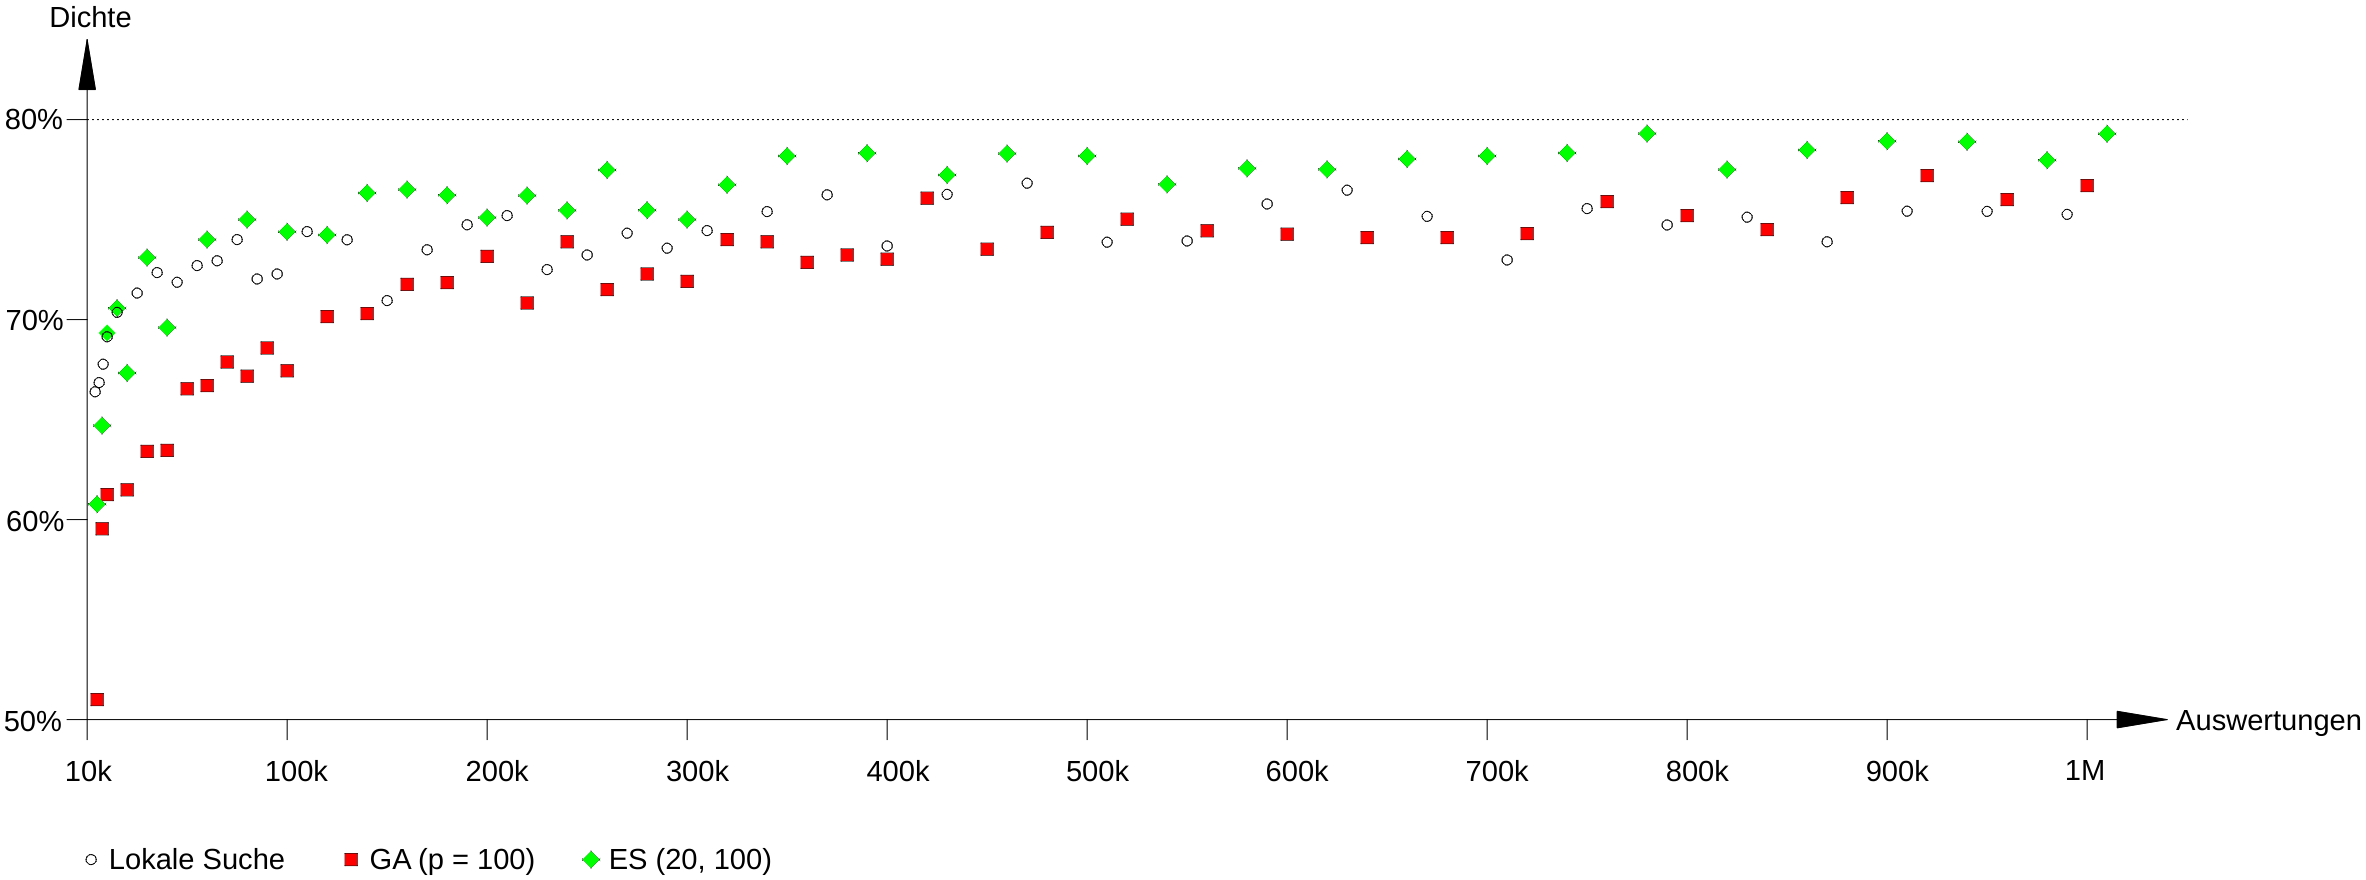
\includegraphics [width=1\textwidth]{Bilder/test_n75.png}
 \caption{
 	Auswertung eines zufälligen Problems mit $n = 75$ für die verschiedenen Algorithmen und Parametrisierungen..
 	}
 \label{fig:test_n75}
\end{figure}

Die Überlegenheit der Evolutionsstrategie ist hier deutlicher als beim Benchmark-Test zu erkennen.
Der genetische Algorithmus erreicht erst bei einer sehr hohen Anzahl an Auswertungen geringfügig bessere Ergebnisse als die lokale Suche, wobei die Streuung der Ergebnisse gegenüber der lokalen Suche geringer ausfällt. Jedoch erzielt der Genetische Algorithmus durchweg schlechtere Ergebnisse als die Evolutionsstrategie bei einer vergleichbaren Anzahl an Auswertungen.\\

Das Optimum aller Durchläufe wurde mittels der Evolutionsstrategie $(20, 100)$ bei $780.000$ Auswertungen erreicht, und weist eine relative Dichte von $79,3\%$ auf.
Der Phänotyp des gefundenen Individuums ist in Abbildung \ref{fig:optimum_n75} dargestellt.
Wie zu erkennen ist, wäre eine geringfügige zusätzliche Optimierung noch möglich.\\

Bei einer anderen Wahl der Kreisradien konnten teilweise relative Dichten von über $84\%$ beobachtet werden.
Die zufällige Zusammenstellung der Kreisradien im Testfall beinhaltet eine hohe Menge an verhältnismäßig großen Kreisen, was eine extrem dichte Anordnung erschwert.

\begin{figure}[H]
 \centering
 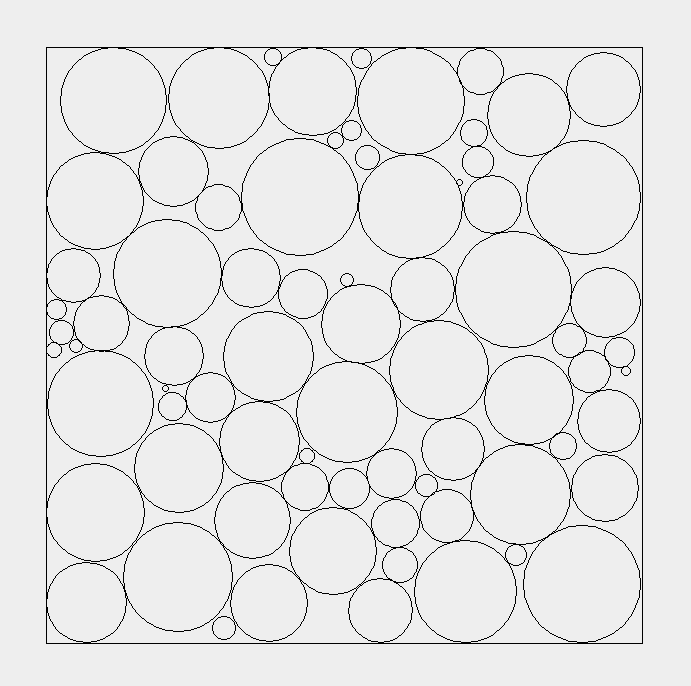
\includegraphics [width=0.5\textwidth]{Bilder/best_n75.png}
 \caption{
 	Bestes gefundenes Individuum über alle Durchläufe des Zufallsproblems mit $n = 75$.
 	Ergebnis der Evolutionsstrategie $(20, 100)$ bei $780.000$ Auswertungen und einer relativen Dichte von $79,3\%$.
 	}
 \label{fig:optimum_n75}
\end{figure}

\nsecend%{Test mit Zufallsdaten}

\nsecbegin{Fazit}

Alle realisierten Ansätze führen bei guter Parametrisierung zu brauchbaren Ergebnissen.
Leider scheint ein genetischer Algorithmus für das gewählte Problem, bzw. den gewählten Genotyp, ungeeignet.
Besonders überzeugend sind die Ergebnisse der Evolutionsstrategie, welche zuverlässig deutlich bessere Lösungen erzielt als lokale Suche und genetischer Algorithmus.\\

Das Projekt ist insgesamt enorm lehrreich und bietet einen angenehmen Schwierigkeitsgrad.
Die grafische Darstellung des Phänotyps des aktuell besten Individuum in der \gls{GUI} erwies sich als äußerst hilfreich, sei es zum Debuggen oder zur menschlichen Beurteilung der Ergebnisse.

\nsecend%{Fazit}

\nsecend%{Auswertung der finalen Implementierungen}

%%%%%%%%%%%%%%%%%%%%%%%%%%%%%%%%%%%%%%%%%%%%%%%%%%%%%%%%%%%%%%%%%%%%%%%%%%%%%%

\nsecbegin{Hinweise zur Implementierung}

Das Projekt wurde in Java 1.8 realisiert und nutzt Java Swing zur Darstellung einer einfachen \gls{GUI}.
Es wurde unter Ubuntu 18.04 mit Oracle Java 13.0.2 getestet, sollte jedoch auch unter anderen Versionen lauffähig sein.\\

Einige der wichtigsten Parameter können über die Menüleiste der \gls{GUI} eingestellt werden.
Nach einer Änderung der Problemgröße $n$ muss der Algorithmus neu mit $n$ zufälligen Radien initialisiert werden, was mittels des Buttons ''Init'' durchgeführt werden kann.
Die konfigurierte Suche für die festgelegte Gesamtzahl an Generationen kann über den Button ''Start'' gestartet werden.
Das Eingabefeld ''Delay'' erlaubt es, nach jeder Änderung des Phänotyps in der Hauptansicht eine Wartezeit in Millisekunden festzulegen, um eine verlangsamte Beobachtung des Algorithmus zu ermöglichen.
In der Fußleiste des Hauptfensters werden Daten der aktuellen Suche angezeigt.
Die Felder ''best score'' und ''density'' beziehen sich hierbei jeweils auf das beste Individuum der aktuellen Generation.\\

Im zweiten Tab der \gls{GUI} wird die Zeitreihe der aktuellen Suche aufgezeichnet.
Jeder Datenpunkt repräsentiert hierbei ebenfalls das beste Individuum der jeweiligen Generation.\\

Eine Darstellung der \gls{GUI}-Ansicht ist in Abbildung \ref{fig:gui} zu finden.

\begin{figure}[h]
 \centering
 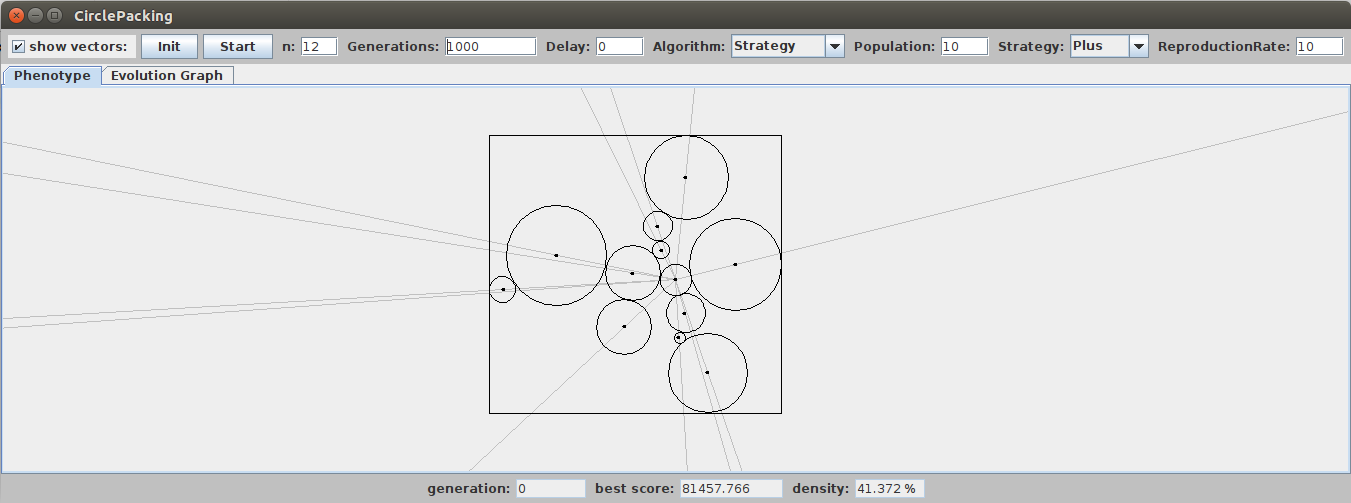
\includegraphics [width=1\textwidth]{Bilder/gui.png} \\
 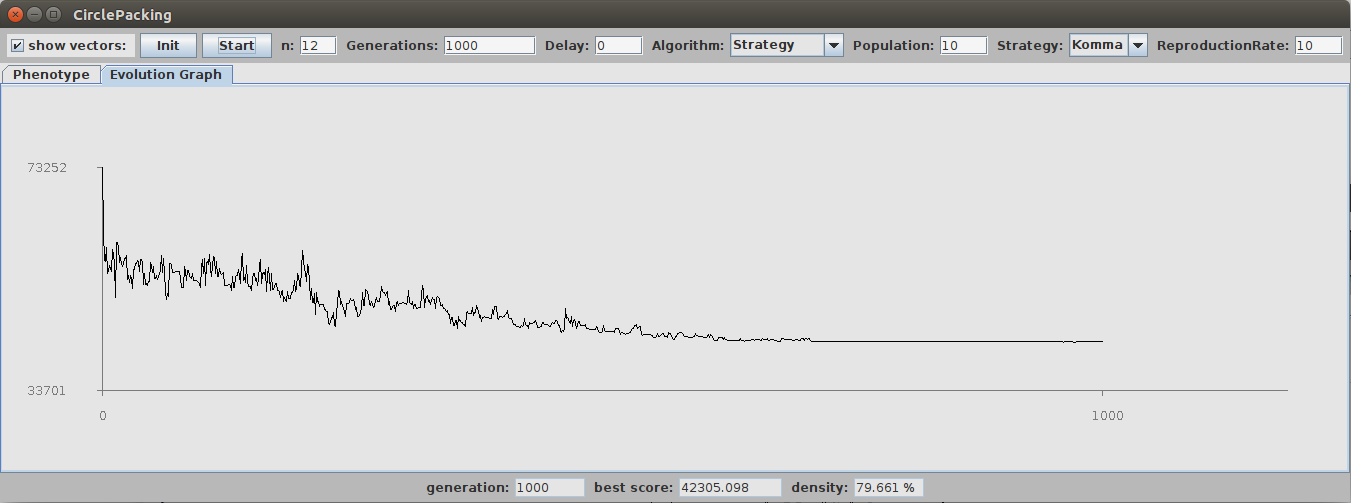
\includegraphics [width=1\textwidth]{Bilder/gui2.png}
 \caption{
 	Screenshot der \gls{GUI} mit Darstellung des aktuell besten Phänotyps (Oben)
 	sowie der aktuell aufgenommenen Zeitreihe (Unten).
 	}
 \label{fig:gui}
\end{figure}

Der Quellcode des Projekts ist unter anderem im GIT-Repository unter \url{https://github.com/Luftschlosser/EvolutionaryCirclePacking} zu finden und ist zur Wiederverwendung freigegeben.
Allerdings finden sich definitiv einige Bugs in der Implementierung, da diese schnell entwickelt und nur oberflächlich getestet wurde.

\nsecend%{Hinweise zur Implementierung}

%%%%%%%%%%%%%%%%%%%%%%%%%%%%%%%%%%%%%%%%%%%%%%%%%%%%%%%%%%%%%%%%%%%%%%%%%%%%%%

%Fazit: Strategy best
%Hinweis zur Implementierung: Java, Gui.

% % % END % % %


%Ende der nsec-Makros 
%(Dient zur überprüfung ob alle sections geschlossen wurden)
\nsecdocumentend

%%%%%%%%%%%%%%%%%%%%%%%%%%%%%%%%%%%%%%%%%%%%%%%%%%%%%%%%%%%%%%%%%%%%%%%%%%%%%%
\printglossary[title=Glossar] %glossar anzeigen
%%%%%%%%%%%%%%%%%%%%%%%%%%%%%%%%%%%%%%%%%%%%%%%%%%%%%%%%%%%%%%%%%%%%%%%%%%%%%%
%Abkürzungen ausgeben
\printglossary[type=\acronymtype,title=Abkürzungsverzeichnis]
%%%%%%%%%%%%%%%%%%%%%%%%%%%%%%%%%%%%%%%%%%%%%%%%%%%%%%%%%%%%%%%%%%%%%%%%%%%%%%
%Bib-Verzeichniss (Zitate) ausgeben
\printbibliography


\end{document}
